\documentclass[11pt]{article}

\usepackage[utf8]{inputenc}
\usepackage[T1]{fontenc}
\usepackage[margin=1in]{geometry}
\usepackage{amsmath}
\usepackage{amssymb}
\usepackage{graphicx}
\usepackage{booktabs}
\usepackage{caption}
\usepackage{placeins}
\usepackage{authblk}
\usepackage{xcolor}
\usepackage[colorlinks=true,linkcolor=blue,citecolor=blue,urlcolor=blue]{hyperref}

\graphicspath{{figures/}}
 
% Convenient shorthands for the moments
\newcommand{\muG}{\mu_G}
\newcommand{\muR}{\mu_R}
\newcommand{\sigGsq}{\sigma_G^2}
\newcommand{\sigRsq}{\sigma_R^2}
\newcommand{\CRG}{C_{RG}}
\newcommand{\kon}{k_{\mathrm{on}}}
\newcommand{\koff}{k_{\mathrm{off}}}
\newcommand{\ksyn}{k_{\mathrm{syn}}}
\newcommand{\kdeg}{k_{\mathrm{deg}}}
\newcommand{\E}{\mathbb{E}}

\title{\textbf{The Telegraph Model of Gene Expression:\\
A Triangular Cross-Validation of Stochastic Simulation}}

\author{Zakhar Guzii}
\affil{Kyiv School of Economics, Department of Mathematics\\
\texttt{zakharguzii@gmail.com}}
\date{June 2026}

\begin{document}

\maketitle

\begin{abstract}
Gene expression---the process by which a gene's DNA is read out to make messenger
RNA (mRNA), the molecule that carries its instructions---is a stochastic process:
even genetically identical cells in the same environment produce very different
numbers of mRNA molecules. The telegraph model explains the main source of this
variability. It treats a gene as a two-state (ON/OFF) switch that transcribes mRNA
only while active. We study the telegraph model in three independent ways and check
that all three agree: we (i) generate stochastic trajectories with the Gillespie
stochastic simulation algorithm (SSA); (ii) derive and solve a closed system of
ordinary differential equations (ODEs) for the first and second moments; and
(iii) draw independent samples directly from the analytic steady-state
distribution, using the classic Beta--Poisson law together with an explicit
Bernoulli gene state. The main
contribution is the cross-validation that links the three methods. The code is available at
\url{https://github.com/zakhar-guzii/telegraph-model-gene-expression}.
\end{abstract}

\section{Introduction}

A surprising fact of molecular biology is that gene expression is variable. Two cells with the same DNA, grown together in the same environment, can have different numbers of copies of the same mRNA or protein~\cite{elowitz2002,ozbudak2002}. This difference between cells is called phenotypic noise. It happens naturally because of random molecular interactions. Experimentally this variability
separates into two parts~\cite{elowitz2002}: \emph{extrinsic} noise, caused by differences between
cells---their size, cell-cycle stage, or the pool of available polymerases---and \emph{intrinsic}
noise, the randomness of the transcription and degradation events themselves, which persists even
between two identical copies of a gene inside the \emph{same} cell. The telegraph model studied here
describes the intrinsic component. Inside a cell the key
players---a single copy of the gene, a handful of
transcription factors (regulatory proteins that bind DNA and control gene activity),
a few dozen mRNA molecules---are present in such small numbers that the discreteness
and randomness of individual chemical events cannot be averaged away. The promoter
(the DNA region that controls when a gene is switched on) switches between an active
and an inactive state at random times. While active, it produces mRNA molecules
through transcription (the synthesis of mRNA from the gene's DNA) in random bursts.
Each mRNA molecule is then degraded---broken down and removed---at a random time. As
a result, the mRNA count is a discrete-valued stochastic process, not a
deterministic quantity.

The telegraph model is the simplest framework that reproduces this behaviour. It
idealises the gene as a two-state device---like a telegraph key that is either
pressed (ON) or released (OFF)---that produces mRNA only while ON~\cite{ko1991}. Despite its
simplicity, it reproduces the bursty, \emph{over-dispersed} mRNA distributions seen
in single-molecule experiments, which count individual mRNAs inside single
cells~\cite{raj2006}, and it can be analysed exactly~\cite{peccoud1995}. A
convenient way to measure this spread is the \emph{Fano factor} $F=\sigma^2/\mu$~\cite{fano1947},
the ratio of the variance to the mean of the mRNA count. Pure Poisson production and
decay, in which every event is independent, has variance equal to mean, giving the
\emph{Poisson baseline} $F=1$. ``Over-dispersed'' means $F>1$: the random switching of
the gene adds extra variability on top of that baseline.

We treat the telegraph model as a case study in how a stochastic process can be
described from several mathematically distinct viewpoints. We implement three
approaches that look unrelated:

\begin{enumerate}
  \item a stochastic simulation (the SSA), which answers ``what does a single cell
    actually do?'';
  \item a system of moment ODEs, which answers ``what does the average cell do, and
    how spread out is the population?'';
  \item a steady-state sampler, which answers ``what does the population look like
    after a very long time?''.
\end{enumerate}

Each approach is correct by itself. But only by comparing them can we be sure that
all three are built correctly and that our understanding of the model is right.

\section{Model Formulation}
\label{sec:model}

The state of the system at time $t$ is the pair
\begin{equation}
  \big(G(t),\,R(t)\big), \qquad G(t)\in\{0,1\}, \quad R(t)\in\mathbb{N},
\end{equation}
where the binary variable $G$ records whether the gene is OFF ($G=0$) or ON
($G=1$), and the integer $R$ counts the number of mRNA molecules present. Four basic reactions define the dynamics of the system. Each reaction has a \emph{propensity} $a_j$, the rate at which it fires at any given moment:

\begin{center}
\begin{tabular}{llll}
\toprule
\textbf{Reaction} & \textbf{Description} & \textbf{Effect} & \textbf{Propensity} \\
\midrule
$R_1$ & Gene activation   & $G:0\to1$       & $a_1 = \kon\,(1-G)$ \\
$R_2$ & Gene inactivation & $G:1\to0$       & $a_2 = \koff\,G$ \\
$R_3$ & RNA synthesis     & $R\to R+1$      & $a_3 = \ksyn\,G$ \\
$R_4$ & RNA degradation   & $R\to R-1$      & $a_4 = \kdeg\,R$ \\
\bottomrule
\end{tabular}
\end{center}

All four rate constants are positive. The switching rates $\kon,\koff$ set how quickly
the promoter turns on and off, and their ratio fixes the long-run fraction of time the
gene is active; the factor $G$ in $a_3$ shuts transcription off entirely when the gene
is OFF; and $\kdeg$ is a per-molecule decay rate, so the total degradation propensity
$\kdeg R$ grows with the amount of mRNA present. Together the rates
$(\kon,\koff,\ksyn,\kdeg)$ and an initial condition $(g_0,r_0)$ at time $t_0$ fully
determine the law of the process.

\paragraph{Burst size.}
One derived quantity is used repeatedly below and follows in a line. Once the gene is ON, the only
reaction that can switch it off fires at the constant rate $\koff$, so the duration of an active
period is exponential with mean $1/\koff$; during that period transcription fires at rate $\ksyn$.
The mean number of transcripts made per active period---the \emph{burst size} $B$---is therefore
\begin{equation}
\label{eq:burst}
  B = \ksyn\,\E[\text{ON duration}] = \frac{\ksyn}{\koff}.
\end{equation}
Bursts of this kind are observed directly in single cells~\cite{golding2005,raj2006}, and the exact
consequences of promoter switching for the mRNA distribution, including the limits recovered in
Section~\ref{sec:res-explore}, are worked out in~\cite{iyerbiswas2009}.

Because each waiting time is exponential and depends only on the current state,
$(G(t),R(t))$ is a continuous-time Markov chain (CTMC): a process that jumps between
discrete states, with the next state depending only on the present one. Its
distribution $P_t(g,r)=\Pr\{G(t)=g,\,R(t)=r\}$ evolves according to the chemical
master equation~\cite{vankampen,gardiner,wilkinson,ingalls}
\begin{equation}
\label{eq:master}
\begin{aligned}
  \frac{\mathrm{d}}{\mathrm{d}t} P_t(g,r)
  ={}& \kon\big[\delta_{g,1}P_t(0,r) - \delta_{g,0}P_t(g,r)\big] \\
   &+ \koff\big[\delta_{g,0}P_t(1,r) - \delta_{g,1}P_t(g,r)\big] \\
   &+ \ksyn\,\delta_{g,1}\big[P_t(1,r-1) - P_t(1,r)\big] \\
   &+ \kdeg\big[(r+1)P_t(g,r+1) - r\,P_t(g,r)\big],
\end{aligned}
\end{equation}
with the convention $P_t(g,-1)=0$. Equation~\eqref{eq:master} underlies all three approaches below: the SSA samples trajectories whose distribution solves it, the moment ODEs are derived from it exactly, and the steady-state sampler draws from its $t\to\infty$ fixed point.

\section{Methods}
\label{sec:methods}

\subsection{Stochastic Simulation (Gillespie SSA)}
\label{sec:ssa}

The \emph{stochastic simulation algorithm} (SSA) of
Gillespie~\cite{gillespie1976,gillespie1977,gillespie2007} generates statistically
exact sample paths of a CTMC, making no approximation to the master
equation~\eqref{eq:master}. Its key idea is that, given the current state, two
questions separate: when does the next reaction occur, and which reaction is it?
With $a_0=\sum_{j=1}^{4} a_j$ the \emph{total propensity}, the waiting time is
$\tau\sim\mathrm{Exp}(a_0)$ and reaction $j$ fires with probability $a_j/a_0$.

Our implementation draws these by inversion, using two independent uniforms
$r_1,r_2\sim\mathrm{U}(0,1)$ per step:
\begin{equation}
  \tau = \frac{1}{a_0}\,\ln\!\frac{1}{r_1},
  \qquad
  j = \min\Big\{ k : \textstyle\sum_{i=1}^{k} a_i > r_2\,a_0 \Big\}.
\end{equation}
The time is then advanced by $\tau$, the state updated by reaction $j$, the reaction
propensities recomputed, and the loop repeats for a fixed number of events
$n_{\mathrm{sim}}$. If the total propensity reaches $a_0=0$, no reaction can
fire, so the state is absorbing and is held fixed afterwards.

A single trajectory is the history of one cell. To obtain population statistics, we run $N_{\mathrm{rep}}$ independent trajectories with identical parameters and
average over them. Each trajectory advances by its own random time increments, so the same event index occurs at different times in different trajectories. We therefore resample every trajectory onto a shared uniform time grid by a zero-order hold before averaging; the state is piecewise constant between events, so this introduces no error. The empirical moments are then ensemble averages at each grid time, for example
\begin{equation}
\label{eq:ssa-mean}
  \widehat{\muR}(t)
  = \frac{1}{N_{\mathrm{rep}}}\sum_{i=1}^{N_{\mathrm{rep}}} R_i(t),
  \qquad
  \widehat{\muG}(t)
  = \frac{1}{N_{\mathrm{rep}}}\sum_{i=1}^{N_{\mathrm{rep}}} G_i(t),
\end{equation}
with sample variances and the sample gene--RNA covariance defined analogously.

\paragraph{Simulation horizon.}
The loop counter $n_{\mathrm{sim}}$ bounds the number of \emph{events}, not the elapsed time, so an
ensemble has no common end time. We therefore take the shared grid no further than the
earliest-finishing trajectory, $t_{\mathrm{end}}=\min_i t_i^{\,\text{last}}$: extending past that
point would freeze the exhausted trajectories at their final state and bias the ensemble toward
whatever those particular cells happened to be doing when they ran out of events. Each figure
therefore ends at its own, seed-dependent time, in every case a large multiple of the relaxation
time.

Figure~\ref{fig:single-cell} shows what the algorithm produces for a single cell at the reference
parameters $\kon=\koff=0.5$, $\ksyn=20$, $\kdeg=1$: the gene switches ON and OFF at random times,
mRNA accumulates in bursts while it is ON, and each burst then decays away. Averaging
$N_{\mathrm{rep}}=1000$ such trajectories according to~\eqref{eq:ssa-mean} gives the ensemble
moments that Section~\ref{sec:res-ssa-ode} compares with the moment ODEs of Section~\ref{sec:ode}.

\begin{figure}[htbp]
  \centering
  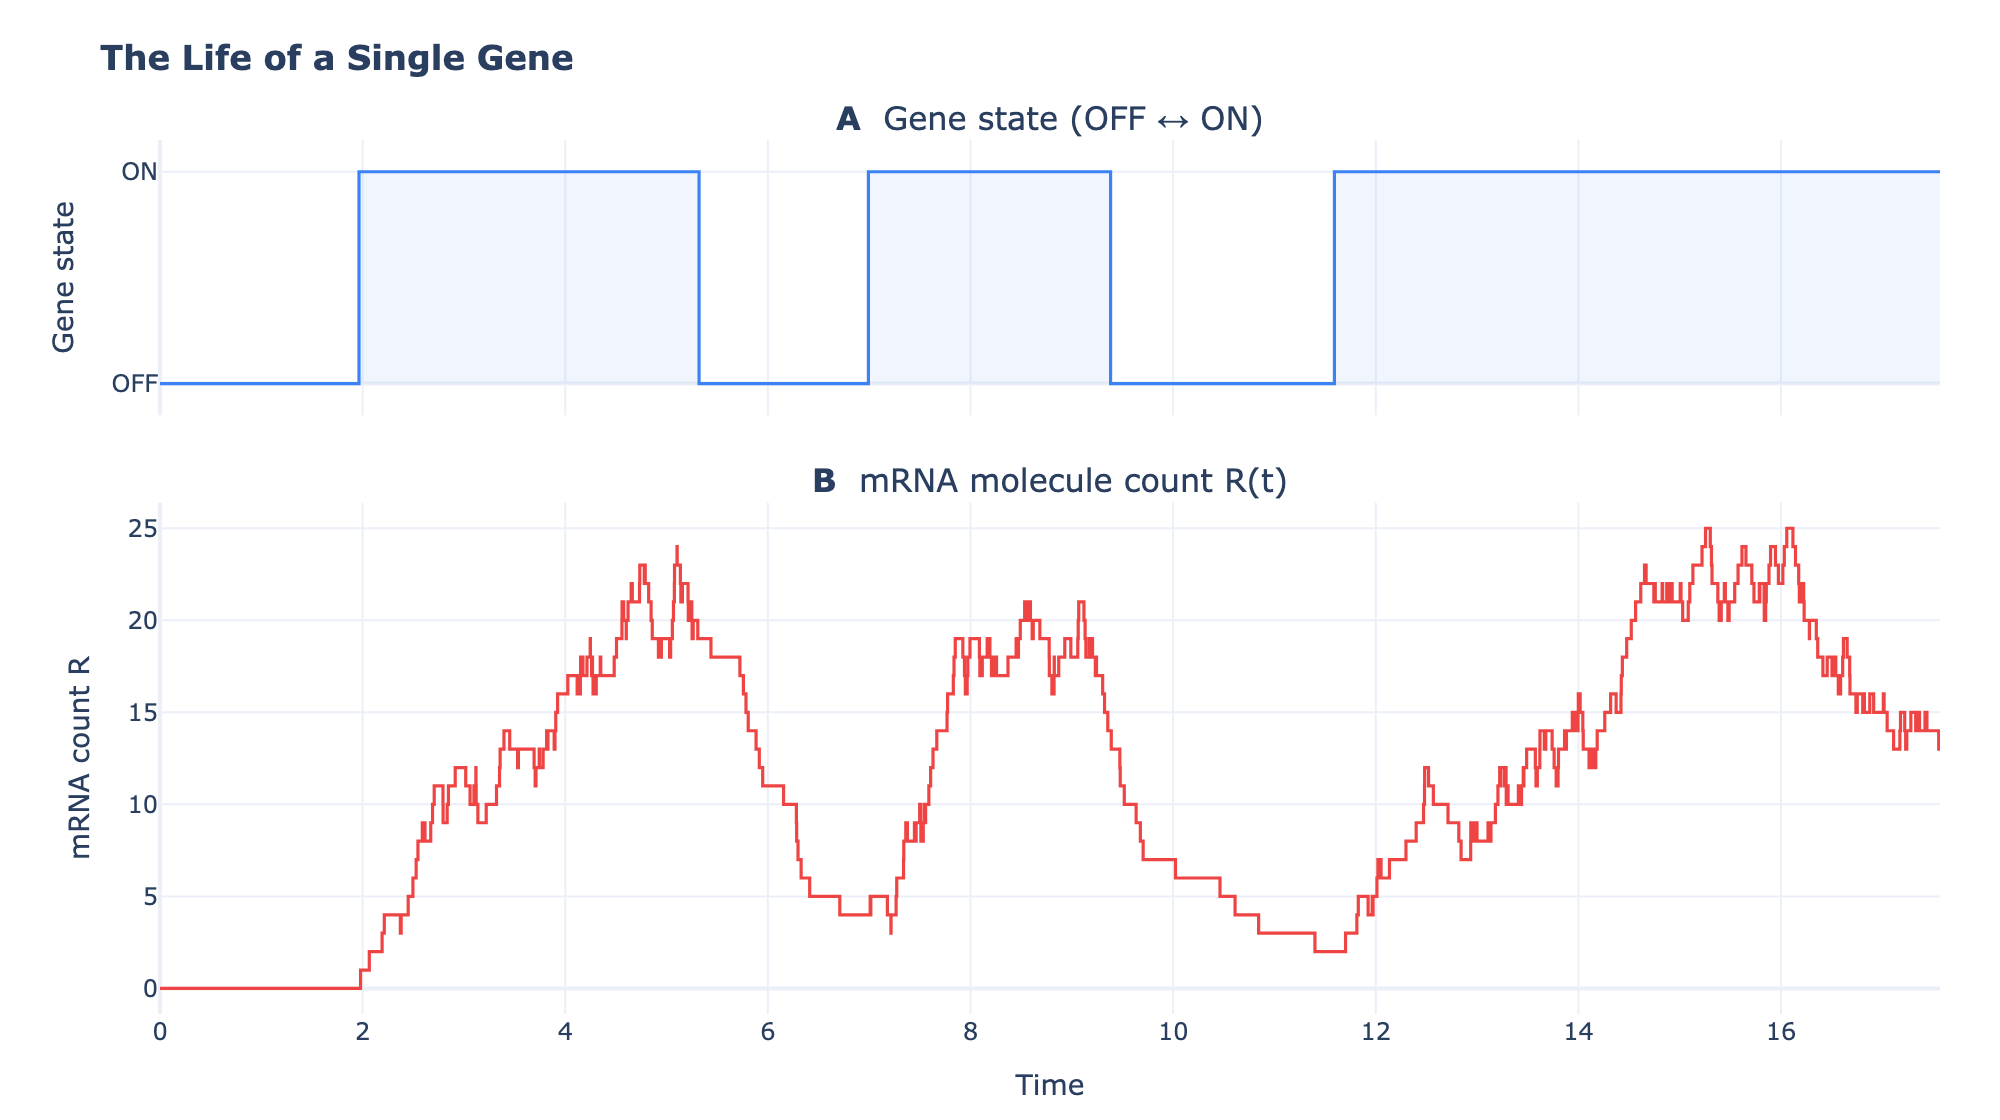
\includegraphics[width=0.85\textwidth]{single_cell_trajectory.png}
  \caption{One stochastic run, i.e.\ a single sample path (``the life of a single gene''), at
    $\kon=\koff=0.5$, $\ksyn=20$, $\kdeg=1$. Top: the gene state switches
    between OFF and ON at random times. Bottom: the mRNA count rises in bursts during ON periods and
    decays between them. Averaging many such trajectories gives the sample moments used below.}
  \label{fig:single-cell}
\end{figure}

\paragraph{Random number generation.}
All experiments draw from the Mersenne Twister~\cite{matsumoto1998} in its MT19937 form, as supplied
by \texttt{numpy.random}~\cite{harris2020}, with a seed fixed for each experiment.

\subsection{Moment ODEs}
\label{sec:ode}

The SSA describes individual cells. Often we instead want deterministic equations for population-level statistics---the \emph{moments}. A moment is an expectation: the mean $\muR=\E[R]$ is the average mRNA level, the variance
$\sigRsq=\E[R^2]-\E[R]^2$ measures the spread (the noise), and the covariance
$\CRG=\E[RG]-\E[R]\E[G]$ measures how gene activity and mRNA level vary together.

Applying the standard moment rule for a chemical master equation---the expected rate of
change of any observable is the sum over reactions of each propensity times the change it
makes---to $f=G,R,R^2,GR$ in turn yields four coupled equations for the telegraph
model~\cite{ingalls,wilkinson}:
\begin{align}
\label{eq:dmuG}
  \frac{\mathrm{d}\muG}{\mathrm{d}t} &= \kon\,(1-\muG) - \koff\,\muG , \\
\label{eq:dmuR}
  \frac{\mathrm{d}\muR}{\mathrm{d}t} &= \ksyn\,\muG - \kdeg\,\muR , \\
\label{eq:dsigR}
  \frac{\mathrm{d}\sigRsq}{\mathrm{d}t} &= 2\ksyn\,\CRG - 2\kdeg\,\sigRsq + \ksyn\,\muG + \kdeg\,\muR , \\
\label{eq:dCRG}
  \frac{\mathrm{d}\CRG}{\mathrm{d}t} &= \ksyn\,\sigGsq - (\kon+\koff+\kdeg)\,\CRG .
\end{align}
Each has a direct reading. Activation pushes mean activity toward $1$ and inactivation
pulls it toward $0$; mRNA is made in proportion to the active fraction $\muG$ and removed
in proportion to the amount present; the mRNA variance is driven up by the coupling to
gene activity (the $\CRG$ term) and by the randomness of production and decay, and down by
degradation; and the covariance is created by transcription passing the gene's own
fluctuations $\sigGsq$ on to the mRNA, then damped at the combined rate of switching and
degradation.

\paragraph{Exact closure.}
In a general nonlinear reaction system the equation for each moment depends on higher moments, so
the system never closes and one has to add approximate closure schemes~\cite{schnoerr2015,ingalls,wilkinson}.
Here it closes \emph{exactly}. The only possible nonlinearity is the variance of the gene state,
but because $G$ is binary,
\begin{equation}
\label{eq:closure}
  \sigGsq = \E[G^2]-\muG^2 = \E[G]-\muG^2 = \muG\,(1-\muG),
\end{equation}
which depends on the mean $\muG$ alone. Putting~\eqref{eq:closure} into~\eqref{eq:dCRG} turns the
four equations \eqref{eq:dmuG}--\eqref{eq:dCRG} into a \emph{closed, exact} linear system in
$(\muG,\muR,\sigRsq,\CRG)$, whose solutions are the true moments of the master
equation~\eqref{eq:master}. A four-variable numerical integration is therefore sufficient, with no
closure approximation anywhere in the code.

\paragraph{Implementation.}
The four right-hand sides
\eqref{eq:dmuG}--\eqref{eq:dCRG}, with $\sigGsq$ substituted by~\eqref{eq:closure}, are coded
directly and passed to the explicit Runge--Kutta solver \texttt{scipy.integrate.solve\_ivp}~\cite{virtanen2020}
(method \texttt{RK45}, the embedded Dormand--Prince pair~\cite{dormand1980}) from the initial conditions $\muG(t_0)=g_0$, $\muR(t_0)=r_0$,
$\sigRsq(t_0)=\CRG(t_0)=0$, evaluated on a uniform grid of $1000$ time points. The resulting curves
are exact expectations rather than estimates; Section~\ref{sec:res-ssa-ode} overlays them on the SSA
ensemble at the same rates and the same initial condition.

\paragraph{Steady-state Fano factor.}
Setting the right-hand side of~\eqref{eq:dCRG} to zero gives
$\CRG^{ss}=\ksyn\,\sigGsq/(\kon+\koff+\kdeg)$ with $\sigGsq=\muG^{ss}(1-\muG^{ss})$
by~\eqref{eq:closure}; substituting that into~\eqref{eq:dsigR} at stationarity, where
$2\kdeg\,\sigRsq = 2\ksyn\,\CRG + \ksyn\,\muG + \kdeg\,\muR$ and $\ksyn\muG=\kdeg\muR$
by~\eqref{eq:dmuR}, and dividing by $\muR^{ss}$ yields the Fano factor in closed form:
\begin{equation}
\label{eq:fano}
  F^{ss} \;=\; \frac{\sigRsq}{\muR}\bigg|_{ss}
  \;=\; 1 \;+\; \frac{\ksyn\,\koff}{(\kon+\koff)\,(\kon+\koff+\kdeg)} .
\end{equation}
The additive $1$ is the Poisson baseline: it is what
survives when $\koff\to0$ and the gene stops switching, so the mRNA count is a pure birth--death
process. The second term is the excess contributed by promoter switching, and it vanishes in two
distinct ways---as $\koff\to0$ (the gene is always ON) and as $\kon,\koff\to\infty$ at fixed ratio,
where the denominator grows quadratically while the numerator grows linearly, so a fast-flickering
promoter averages out. Because the decay in that second limit is only $\mathcal{O}(1/\kon)$, the
approach to $F=1$ is slow; Table~\ref{tab:param-exp} quantifies it.

\subsection{Steady-State Sampler}
\label{sec:ss}

As $t\to\infty$ the telegraph model forgets its initial condition and converges to a unique
stationary distribution $P_\infty(g,r)$. Instead of simulating a long transient to reach it, we can
sample from $P_\infty$ directly. Peccoud and Ycart~\cite{peccoud1995} showed that at steady state
the mRNA count follows the classic \emph{Beta--Poisson} law: it is Poisson, but with a mean that is
itself random from cell to cell. Let the \emph{mixing fraction} $p\in[0,1]$ be the long-run share of
time a cell's gene spends ON. Across a population $p$ is Beta-distributed, and given $p$ the mRNA
count is Poisson with mean $\lambda=(\ksyn/\kdeg)\,p$. Here $\ksyn/\kdeg$ is the \emph{transcription
efficiency coefficient}: the mean mRNA level a permanently active gene would reach. With the
dimensionless switching rates $a=\kon/\kdeg$ and $b=\koff/\kdeg$ (so $\kdeg$ fixes the unit of time),
the stationary mRNA law is therefore
\begin{equation}
\label{eq:beta-poisson}
  R \sim \mathrm{Poisson}\!\big((\ksyn/\kdeg)\,p\big), \qquad p \sim \mathrm{Beta}(a,b).
\end{equation}

Writing $c=\ksyn/\kdeg$ for the transcription efficiency and averaging the Poisson kernel over the
Beta density gives the stationary mRNA law in closed form,
\begin{equation}
\label{eq:py-pmf}
  P_\infty(r)
  = \frac{c^{\,r}e^{-c}}{r!}\,
    \frac{\Gamma(a+r)\,\Gamma(a+b)}{\Gamma(a)\,\Gamma(a+b+r)}\;
    {}_1F_1\!\big(b,\;a+b+r;\;c\big),
\end{equation}
where ${}_1F_1$ is Kummer's confluent hypergeometric function. Equation~\eqref{eq:py-pmf} is the
Peccoud--Ycart result~\cite{peccoud1995}; applying Kummer's transformation
${}_1F_1(\alpha,\gamma,z)=e^{z}\,{}_1F_1(\gamma-\alpha,\gamma,-z)$ with $\alpha=b$, $\gamma=a+b+r$,
$z=c$ absorbs the $e^{-c}$ prefactor and returns the equivalent form
${}_1F_1(a+r,\,a+b+r;\,-c)$ in which the law is more often quoted.

We record~\eqref{eq:py-pmf} but do not evaluate it. The mixture~\eqref{eq:beta-poisson} \emph{is}
this distribution---\eqref{eq:py-pmf} is what one obtains by averaging the Poisson kernel over the
Beta density---so sampling the mixture already samples $P_\infty$ exactly, with no discretisation of
the state space, at the cost of three vectorised draws instead of a call to ${}_1F_1$ for every
count. The closed form states what the sampler targets; it is not the algorithm.

Our sampler implements exactly this law, and draws the gene state as an explicit
$\mathrm{Bernoulli}(p)$ so we can also estimate the joint moments of $(G,R)$. For each of the
$N_{\mathrm{rep}}$ samples it draws
\begin{align}
  p &\sim \mathrm{Beta}(a,b),
  &&f(p) = \frac{\Gamma(a+b)}{\Gamma(a)\,\Gamma(b)}\,p^{\,a-1}(1-p)^{\,b-1}, \\[2pt]
  G \mid p &\sim \mathrm{Bernoulli}(p),
  &&\Pr(G=1\mid p)=p,\quad \Pr(G=0\mid p)=1-p, \\[2pt]
  R \mid p &\sim \mathrm{Poisson}(\lambda),
  &&\lambda = \frac{\ksyn}{\kdeg}\,p .
\end{align}
The key point is that the mRNA count $R$ is conditioned on the mixing fraction $p$, \emph{not} on
the current gene state $G$. Given $p$, the gene state and the mRNA count are drawn independently, so
a cell can have $G=0$ and still $R>0$---as in a real cell, where mRNA made during the last active
period outlives the switch to OFF.

\paragraph{Why the joint construction is the right one.}
Peccoud and Ycart give the \emph{marginal} law of $R$, and~\eqref{eq:py-pmf} is that marginal.
Nothing in it fixes how the gene state should be attached, yet the checks below need
$\widehat{\sigma}_G^{\,ss}$ and $\widehat{\CRG}^{\,ss}$, which are properties of the joint law. Two
assumptions above are therefore ours and not quoted: that $G\sim\mathrm{Bernoulli}(p)$ with the same
mixing fraction $p$ that drives the Poisson mean, and that $G$ and $R$ are conditionally independent
given $p$. Both deserve a check, and the covariance provides one, because it can be computed twice
by routes that share nothing.

From the master equation, setting~\eqref{eq:dCRG} to zero and substituting the exact
closure~\eqref{eq:closure} gives
\begin{equation}
\label{eq:crg-cme}
  \CRG^{ss} = \frac{\ksyn\,\sigGsq}{\kon+\koff+\kdeg}
            = \frac{\ksyn\,\muG^{ss}(1-\muG^{ss})}{\kon+\koff+\kdeg} .
\end{equation}
From the sampler's construction, conditional independence gives
$\E[RG]=\E\big[\E[R\mid p]\,\E[G\mid p]\big]=c\,\E[p^2]$ while $\E[R]\E[G]=c\,\E[p]^2$, so
$\CRG = c\,\mathrm{Var}(p)$ with $\mathrm{Var}(p)=ab/\big((a+b)^2(a+b+1)\big)$ the Beta variance.
Substituting $ab/(a+b)^2=\muG^{ss}(1-\muG^{ss})$ and
$a+b+1=(\kon+\koff+\kdeg)/\kdeg$, and $c=\ksyn/\kdeg$, collapses this to
\begin{equation}
  \CRG = \frac{\ksyn}{\kdeg}\cdot\frac{\muG^{ss}(1-\muG^{ss})\,\kdeg}{\kon+\koff+\kdeg}
       = \frac{\ksyn\,\muG^{ss}(1-\muG^{ss})}{\kon+\koff+\kdeg},
\end{equation}
which is~\eqref{eq:crg-cme} term for term. The agreement is symbolic rather than a numerical
coincidence at one parameter set, so the two added assumptions are the ones that make the sampler's
joint moments those of the master equation.

This construction makes a sharp prediction at the edge of parameter space. As the switching rates
become small compared with degradation ($a,b\to0$), the $\mathrm{Beta}(a,b)$ density piles its mass
at the endpoints $p=0$ and $p=1$, and the mixture separates into its building blocks: a single
Bernoulli trial for the gene state and, when ON, an ordinary Poisson count for the mRNA. In
particular at $\koff=0$ the mixing fraction is degenerate, $p\equiv1$, and the stationary law must
collapse to a plain $\mathrm{Poisson}(\ksyn/\kdeg)$. We test that prediction numerically in
Section~\ref{sec:res-ss}.

The joint stationary law is the average of these conditional distributions over the mixing
fraction,
\begin{equation}
  P_\infty(g,r) = \int_0^1 \Pr(G=g\mid p)\,\Pr(R=r\mid p)\,f(p)\,\mathrm{d}p ,
\end{equation}
which our sampler never evaluates directly: drawing $N_{\mathrm{rep}}$ triples $(p,G,R)$ and
averaging gives unbiased Monte Carlo estimates of the steady-state moments
$\widehat{\muG}^{\,ss},\widehat{\muR}^{\,ss}$, and so on. Two edge cases are handled explicitly. If
$\koff=0$ the gene never switches off, so $p$ is fixed at $1$ rather than drawn; if $\kdeg=0$ no
steady state exists (mRNA grows without bound) and the input is rejected. The exact
stationary means used as the reference below are
\begin{equation}
\label{eq:ss-means}
  \muG^{ss} = \frac{\kon}{\kon+\koff},
  \qquad
  \muR^{ss} = \frac{\ksyn}{\kdeg}\,\muG^{ss},
\end{equation}
obtained by setting the time derivatives in~\eqref{eq:dmuG}--\eqref{eq:dmuR} to
zero.

\subsection{The Validation Triangle}
\label{sec:intersection}

The three methods are different mathematical objects, but probability theory
predicts exact relationships between them. We state these as the three edges of a
\emph{validation triangle} and test each one numerically in the experiments that
follow.

\paragraph{Edge 1 --- SSA $\leftrightarrow$ Moment ODEs (finite time).}
The empirical averages~\eqref{eq:ssa-mean} are sample means of independent,
identically distributed trajectories. By the Law of Large
Numbers, as $N_{\mathrm{rep}}\to\infty$ they converge to the true
expectations, which are exactly the solutions of the moment ODEs:
\begin{equation}
  \lim_{N_{\mathrm{rep}}\to\infty}
  \frac{1}{N_{\mathrm{rep}}}\sum_{i=1}^{N_{\mathrm{rep}}} R_i(t) = \muR(t),
\end{equation}
and likewise for $\muG(t)$ and the covariance $\CRG(t)$. This links the
stochastic and deterministic descriptions: with finitely many replicates, the SSA should follow the ODE curves up to a statistical error of order
$1/\sqrt{N_{\mathrm{rep}}}$.

\paragraph{Edge 2 --- Moment ODEs $\leftrightarrow$ Steady-state sampler (long time).}
The stationary distribution is the $t\to\infty$ limit of the dynamics, so the
moment ODEs must approach a fixed point,
\begin{equation}
  \lim_{t\to\infty}\muG(t) = \muG^{ss},
  \qquad
  \lim_{t\to\infty}\muR(t) = \muR^{ss},
  \qquad \text{etc.,}
\end{equation}
which coincides with~\eqref{eq:ss-means}. The independent steady-state sampler must
estimate \emph{these same} values,
\begin{equation}
  \lim_{N_{\mathrm{rep}}\to\infty}
  \frac{1}{N_{\mathrm{rep}}}\sum_{i=1}^{N_{\mathrm{rep}}} R_i^{ss} = \muR^{ss},
\end{equation}
and likewise for $\muG^{ss}$. By the Central Limit Theorem, the sampler's error decays as
$\sigma/\sqrt{N_{\mathrm{rep}}}$, where $\sigma$ is the standard deviation of the
stationary distribution. Observing this $1/\sqrt{N_{\mathrm{rep}}}$ rate confirms
that the sampler is a valid Monte Carlo estimator of the steady-state moments.

\paragraph{Edge 3 --- SSA $\leftrightarrow$ Steady-state sampler (closing the triangle).}
An SSA trajectory run long enough to reach stationarity samples the same
distribution $P_\infty$ as the direct sampler. Hence the long-time plateau of the
SSA moments must agree with both the ODE fixed point and the sampler
estimates. Because both endpoints of this edge emit samples, the claim can be sharpened to the
equality of the full laws, $\hat P^{\mathrm{SSA}}_\infty = \hat P^{\mathrm{smp}}_\infty$, rather
than of their first two moments alone; Section~\ref{sec:res-ss} tests it in total-variation
distance.

\section{Experiments and Results}
\label{sec:results}

The study is organised into three Jupyter notebooks, one for each part of the
validation.

Unless stated otherwise, the dynamic experiments use the symmetric parameters
$\kon=0.5$, $\koff=0.5$, $\ksyn=20.0$, $\kdeg=1.0$ (time measured in mRNA
lifetimes), with $N_{\mathrm{rep}}=1000$ trajectories and initial condition
$(g_0,r_0)=(0,0)$. These give an active fraction $\muG^{ss}=\kon/(\kon+\koff)=0.5$
and steady-state mean mRNA level $\muR^{ss}=(\ksyn/\kdeg)\,\muG^{ss}=10$,
by~\eqref{eq:ss-means}. The five-moment sampler check in
Section~\ref{sec:res-ss} uses $\koff=1$ instead, which gives $\muR^{ss}=6.667$.

\subsection{Parameter Exploration (Notebook 1)}
\label{sec:res-explore}

\paragraph{Aim.}
This part runs the SSA on its own and checks that it reproduces the behaviour we expect when the
gene's parameters change. We vary one mechanism at a time so that each run isolates a single effect;
the parameter values are listed in Table~\ref{tab:param-exp}. The last row deliberately changes both
numerical knobs at once, since neither the ensemble size nor the run length is a mechanism of the
model.

\begin{table}[htbp]
  \centering
  \small
  \begin{tabular}{llccl}
  \toprule
  \textbf{Experiment} & \textbf{Parameters} & $F^{ss}$ & $\widehat{F}$ (SSA) & \textbf{What it isolates} \\
  \midrule
  Slow switching   & $\kon=\koff=0.05$, $\ksyn=20$        & 10.09 & 9.94 & noise at fixed mean \\
  Fast switching   & $\kon=\koff=10$, $\ksyn=20$          & 1.48  & 1.48 & noise at fixed mean \\
  High expression  & $\kon=0.5,\koff=4,\ksyn=56$          & 10.05 & 9.90 & burst size $\approx14$ \\
  Low expression   & $\kon=0.5,\koff=10,\ksyn=30$         & 3.48  & 3.49 & burst size $\approx3$ \\
  Initial cond.\   & $(g_0,r_0)=(0,0)$ vs.\ $(1,15)$      & 9.33  & 9.41 / 9.27 & forgetting the start \\
  Numerical        & $n_{\mathrm{sim}}=1000$ vs.\ $N_{\mathrm{rep}}=224,\,n_{\mathrm{sim}}=5000$
                                                          & 9.33  & 9.48 / 9.40 & estimate quality \\
  \bottomrule
  \end{tabular}
  \caption{The six parameter-exploration runs. Unless shown otherwise $\kdeg=1$ and the base
    switching rates are $\kon=\koff=0.1$; each run reaches the steady-state mean $\muR^{ss}=10$
    except the expression runs, which change it on purpose. $F^{ss}$ is the closed-form steady-state
    Fano factor~\eqref{eq:fano} for those rates; $\widehat{F}=\widehat{\sigma}_R^2/\widehat{\muR}$ is
    measured from the same SSA run the corresponding figure is drawn from, averaged over the last
    fifth of the horizon. Rows with two runs report both.}
  \label{tab:param-exp}
\end{table}

\begin{figure}[htbp]
  \centering
  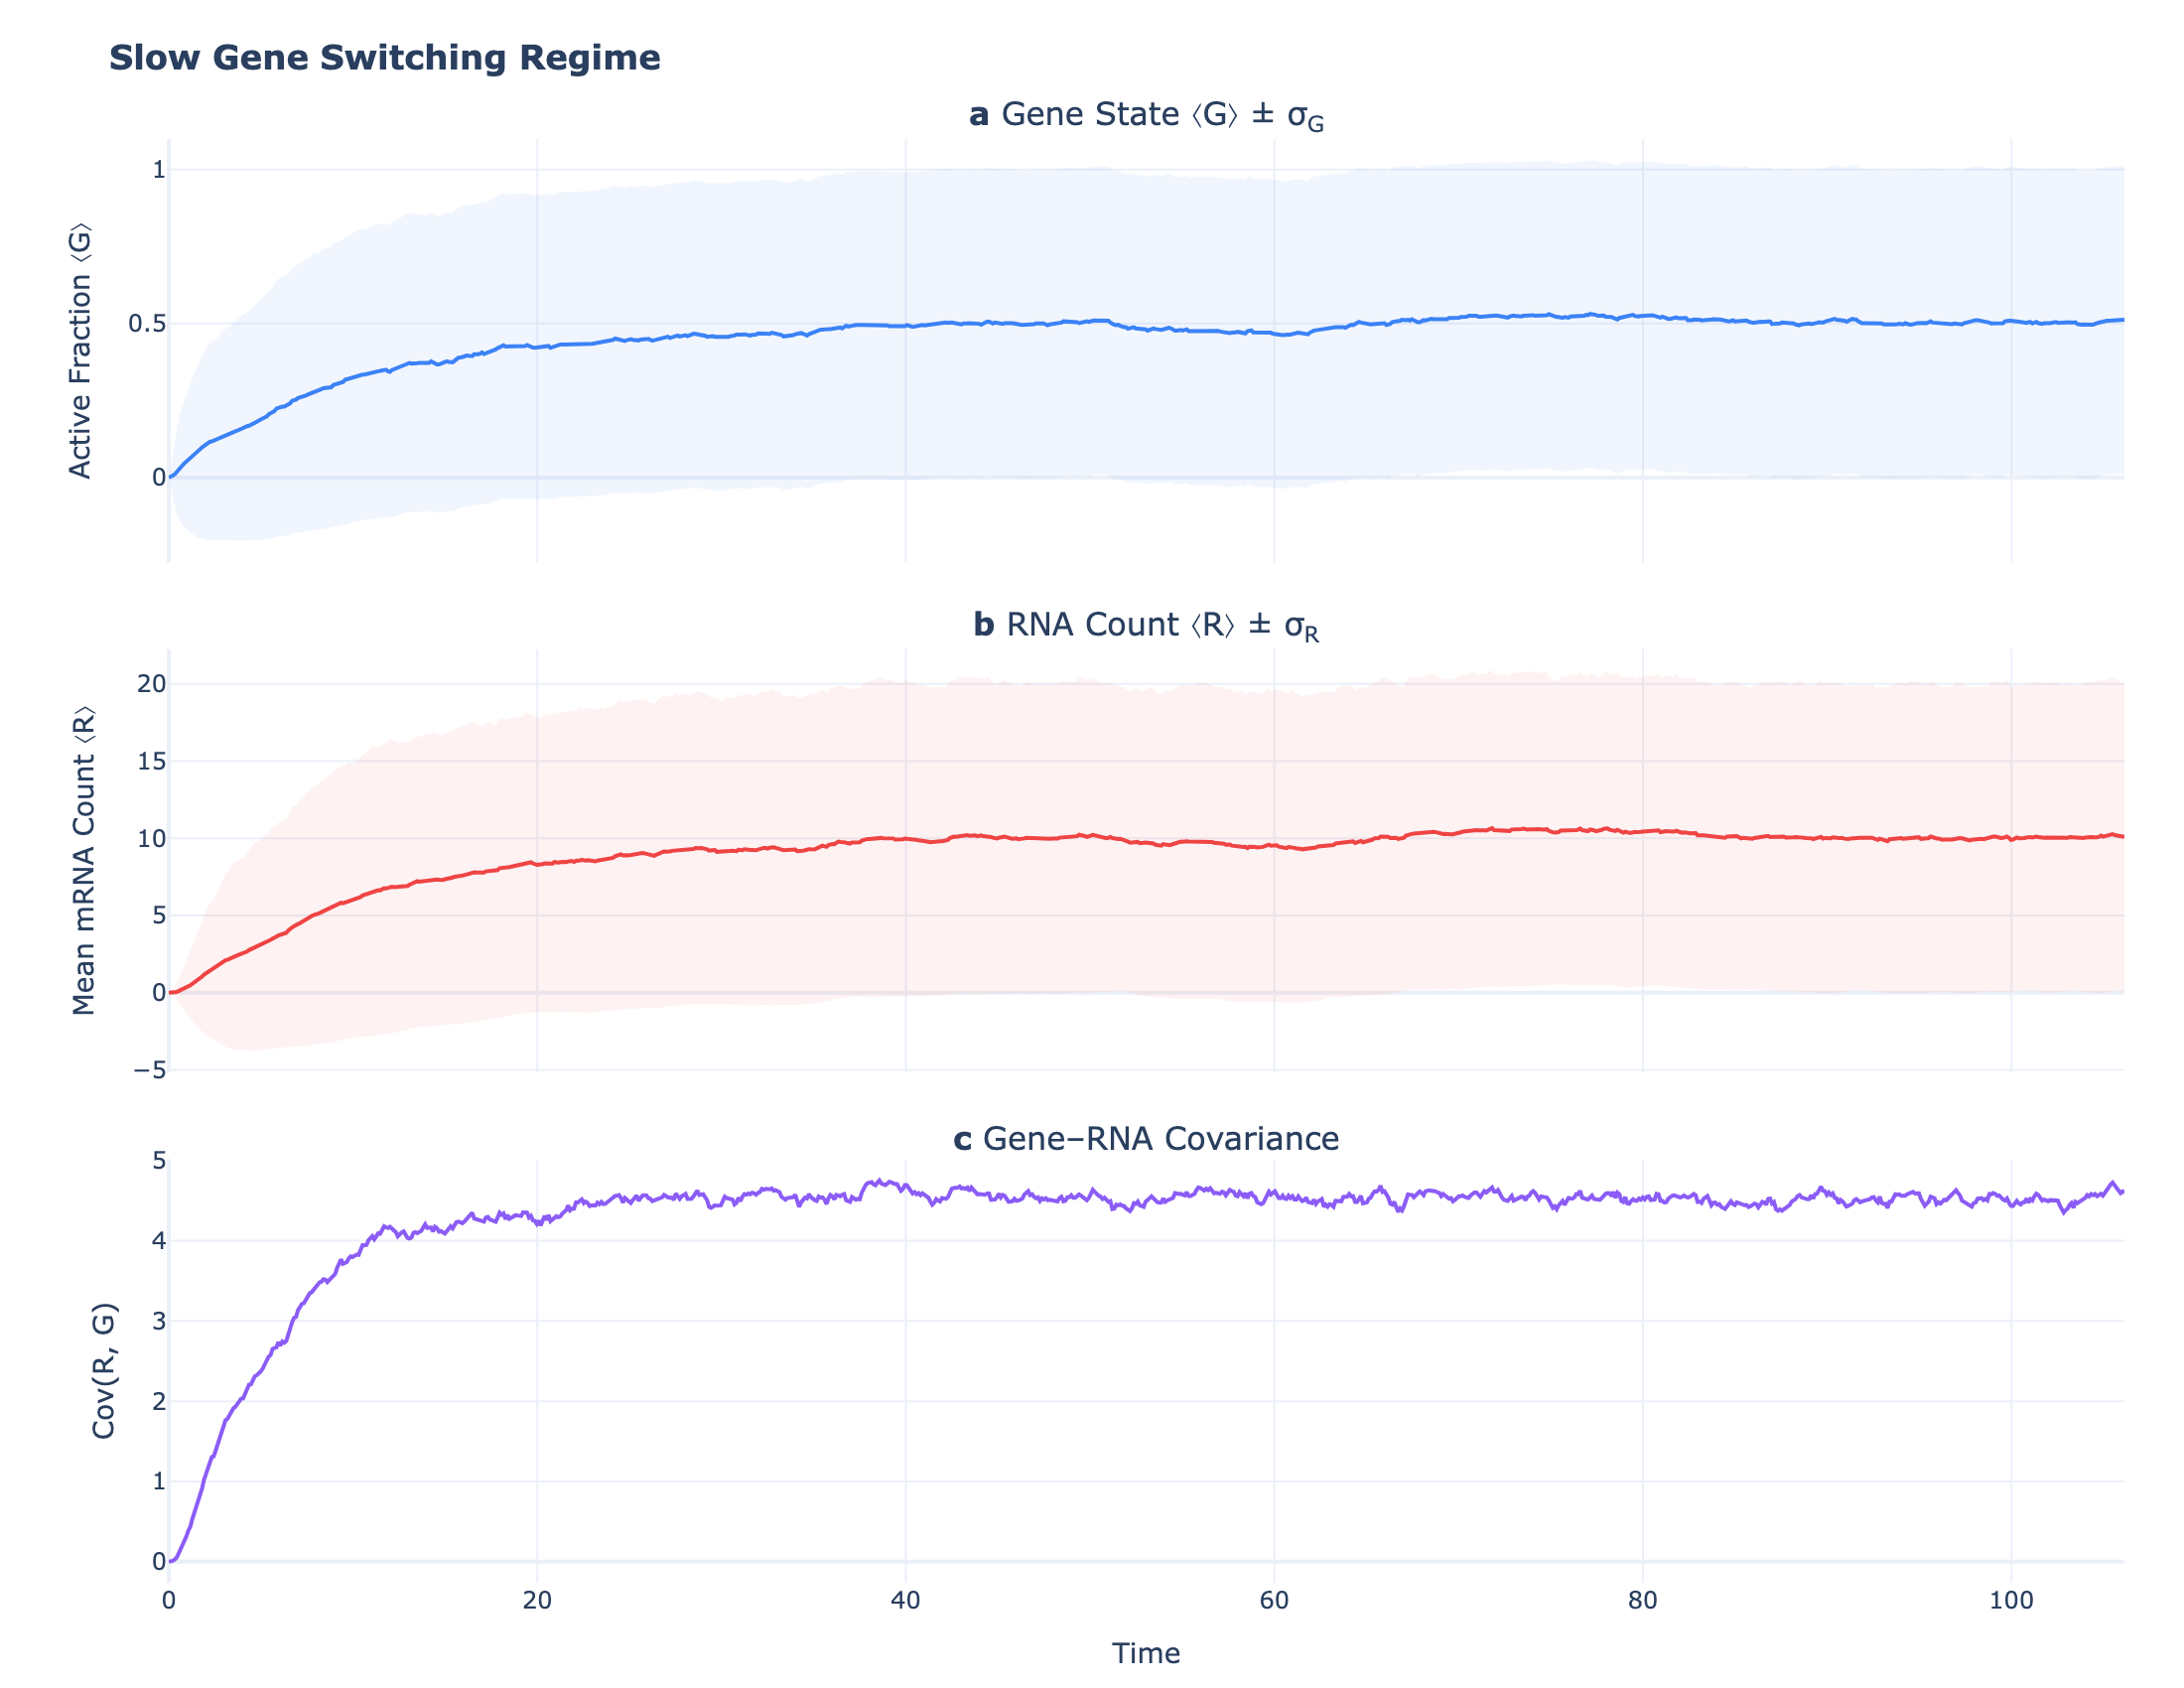
\includegraphics[width=0.49\textwidth]{param_switching_slow.png}
  \hfill
  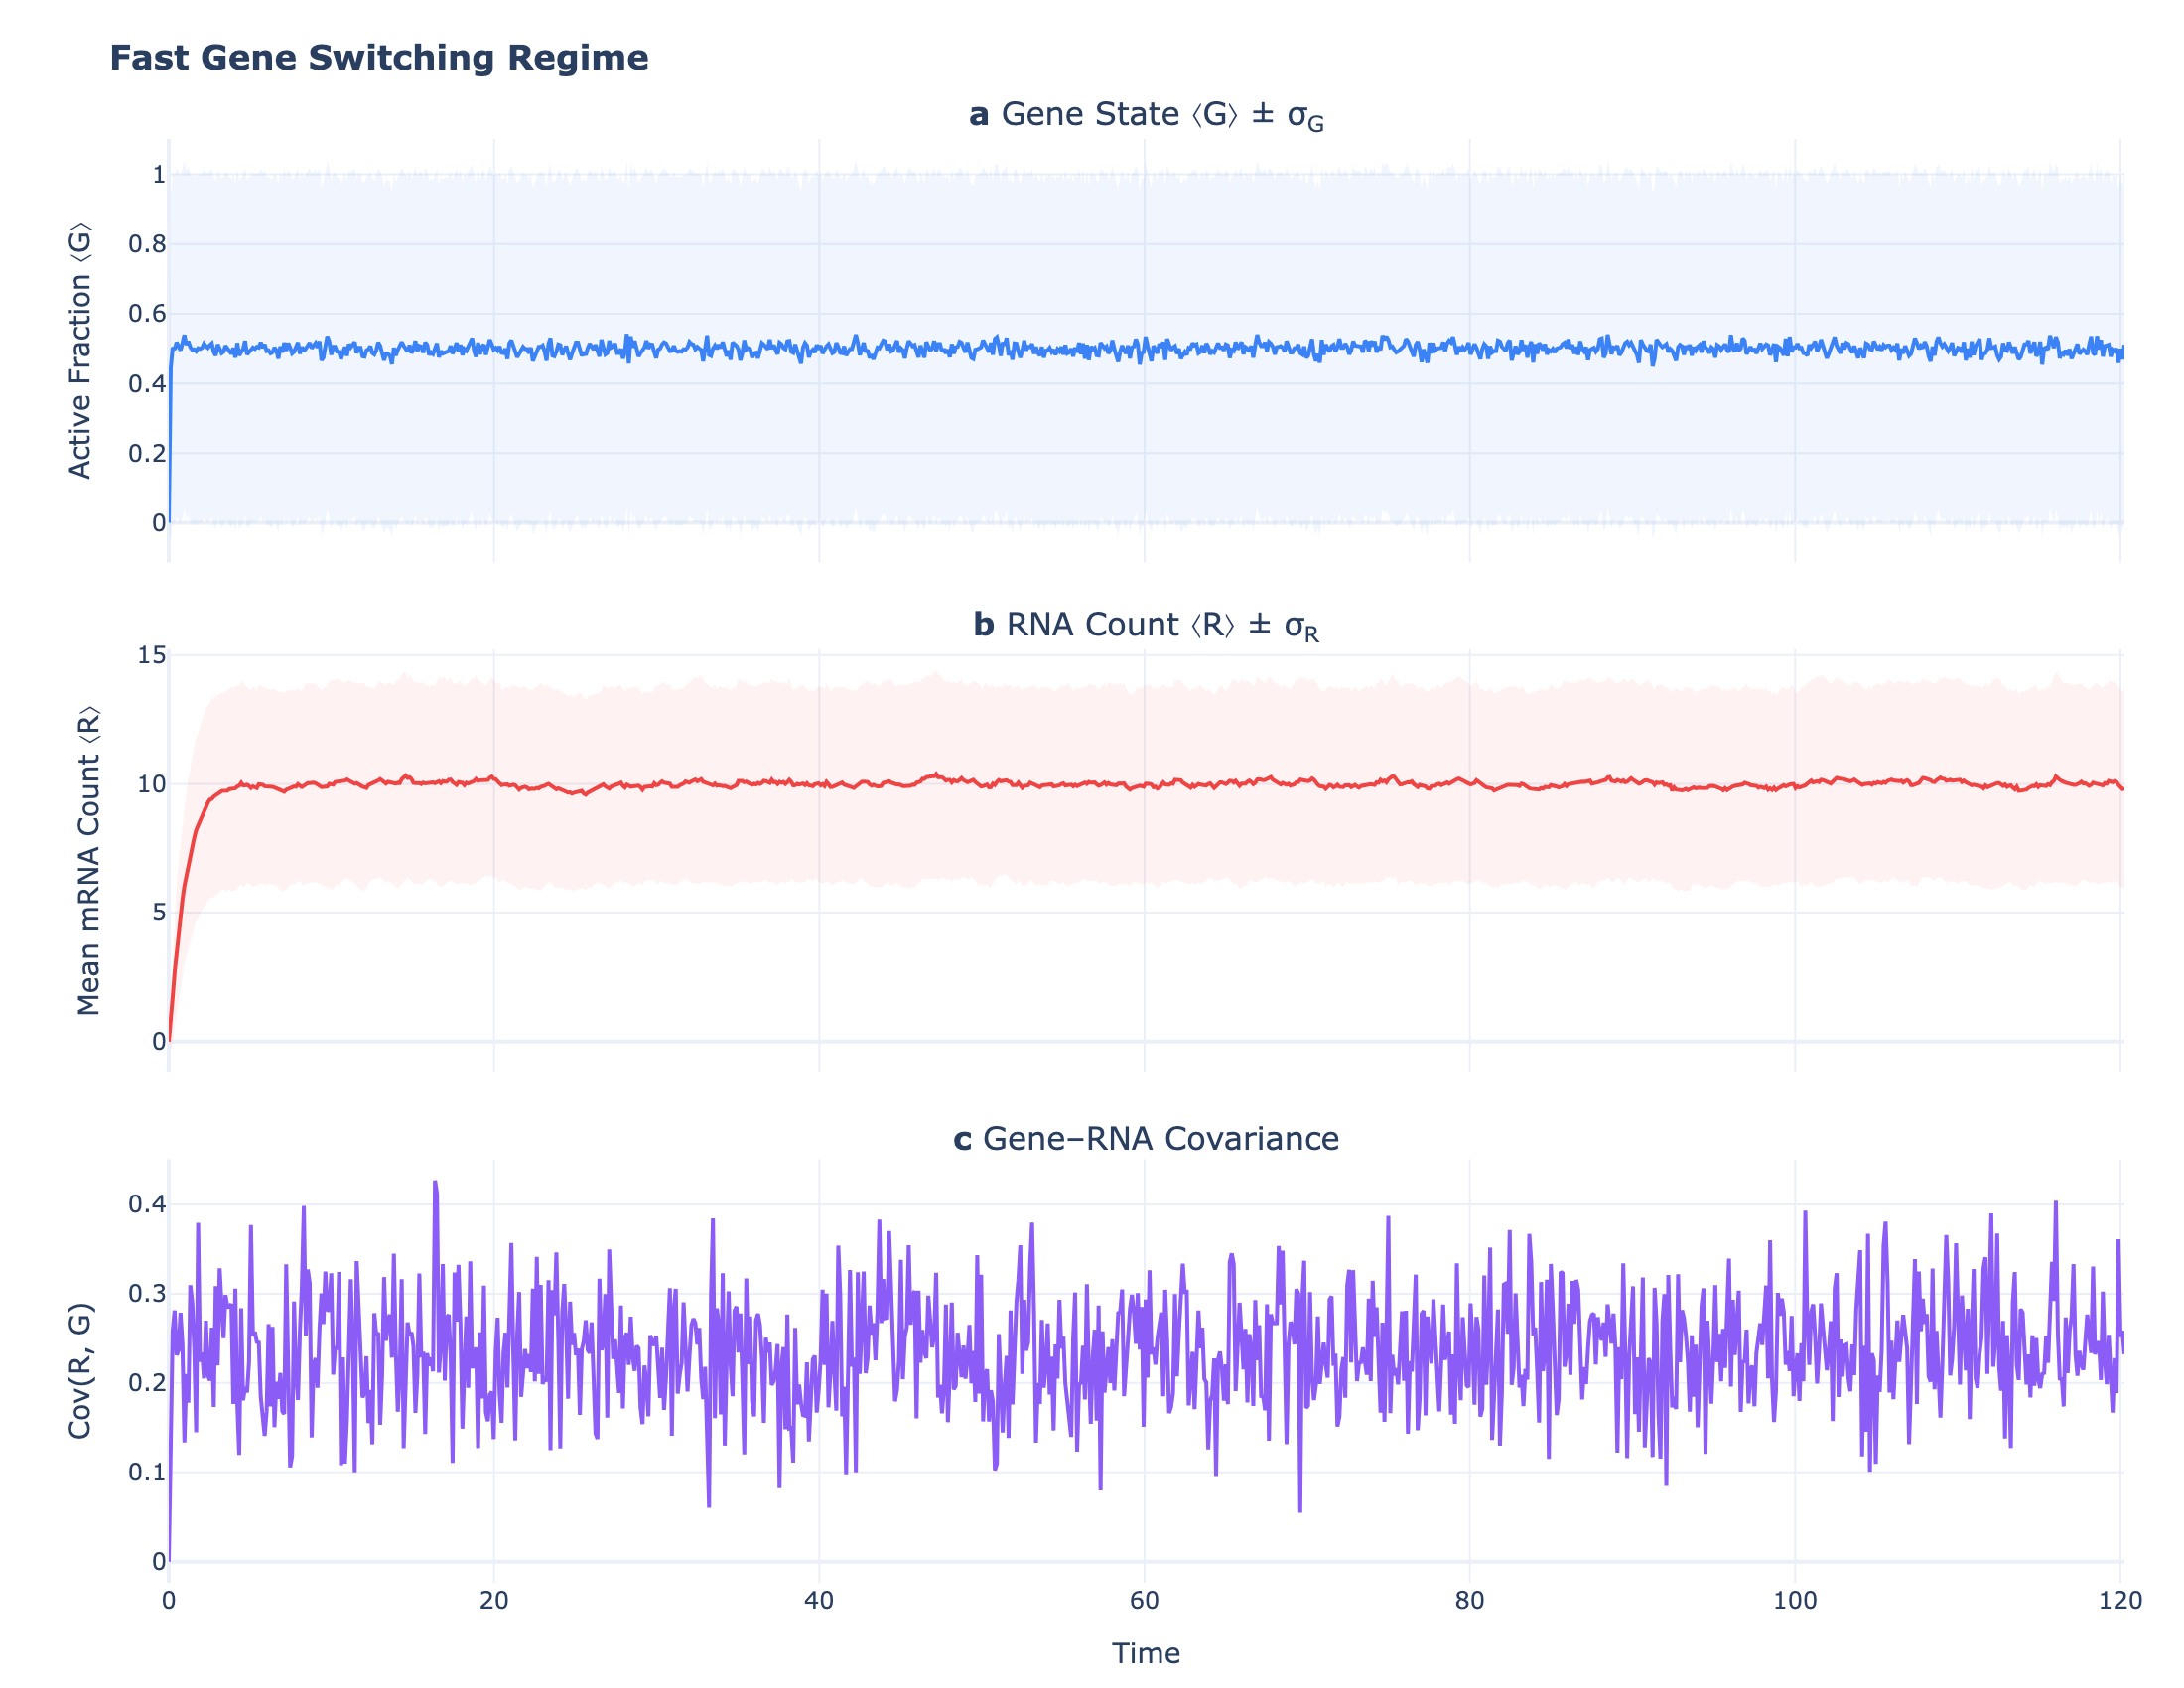
\includegraphics[width=0.49\textwidth]{param_switching_fast.png}
  \caption{Switching speed reshapes noise at fixed mean. Slow switching (left,
    $\kon=\koff=0.05$) gives long bursts, a wide $\pm\sigma_R$ band and strong
    gene--RNA covariance; fast switching (right, $\kon=\koff=10$) flickers so
    quickly that the promoter averages out, leaving a narrow band and near-zero
    covariance. Both reach the same mean $\muR\approx10$.}
  \label{fig:wf-switch}
\end{figure}

\paragraph{Result.}
Three mathematical points come out of these runs. First, switching speed reshapes the noise at a
fixed mean (Figure~\ref{fig:wf-switch}): as $\kon,\koff$ grow relative to $\kdeg$ the gene averages
out, so $\sigRsq$ and $\CRG$ fall and the Fano factor $F=\sigRsq/\muR$ moves toward the Poisson
baseline $F=1$. The closed form~\eqref{eq:fano} says how far it moves and the measured column of
Table~\ref{tab:param-exp} confirms it: from $F^{ss}=10.09$ at $\kon=\koff=0.05$ down to
$F^{ss}=1.48$ at $\kon=\koff=10$. The limit is approached but not reached: at switching ten times
faster than degradation the promoter has not finished averaging out, and by~\eqref{eq:fano} it never
fully does at finite rates, in agreement with the exact analysis of the switching limits
in~\cite{iyerbiswas2009}. Second, the mean is governed by
$\muR^{ss}=(\ksyn/\kdeg)\,\kon/(\kon+\koff)$, so with $\kon$ fixed the burst size~\eqref{eq:burst}
sets how high $\muR$ climbs: the two expression rows of Table~\ref{tab:param-exp} carry $F^{ss}$ from
$10.05$ at burst $\approx14$ to $3.48$ at burst $\approx3$, the weak promoter making few molecules
with a larger \emph{relative} spread (coefficient of variation $\sigma_R/\muR$), which is why
rare-molecule genes look noisier. Third, neither the initial condition nor the numerical resolution
may move the steady state, and neither does: the last four rows of Table~\ref{tab:param-exp} share
the single prediction $F^{ss}=9.33$ and measure between $9.27$ and $9.48$ against it. That the two
initialisations agree confirms the chain is ergodic, and the numerical rows show the estimate---not
the biology---improving, the sampling error scaling as $1/\sqrt{N_{\mathrm{rep}}}$ with extra bias if
runs are too short to reach stationarity. Here $N_{\mathrm{rep}}=224$ is a representative
experiment-scale ensemble, of the order of the cell counts in single-molecule mRNA
studies~\cite{raj2006}. Notebook~1 plots the moment traces behind all six rows.

\paragraph{Conclusion.}
The SSA reproduces every qualitative feature the telegraph model is supposed to have, and where a
closed form exists to check it against---the Fano factor---it reproduces that quantitatively too.
This is the vertex-level check for the simulator: it does not yet compare the SSA with anything
else, which is what Sections~\ref{sec:res-ssa-ode} and~\ref{sec:res-ss} do.

\subsection{SSA vs.\ ODE: Moment Dynamics (Edge 1, Notebook 2)}
\label{sec:res-ssa-ode}

\paragraph{Aim.} Verify that the stochastic simulation and the deterministic moment ODEs
describe the same dynamics at all times (Edge~1 of the validation triangle,
Section~\ref{sec:intersection}). If they agree, the SSA ensemble averages should
track the ODE curves up to sampling noise of order $1/\sqrt{N_{\mathrm{rep}}}$.

\paragraph{Result.}
The direct test is the overlay in Figure~\ref{fig:ssa_vs_ode}, which shows both descriptions of the
same experiment on one set of axes: the same $N_{\mathrm{rep}}=1000$ trajectories and the same
integration, computed by methods that share no code. Starting from a
silent gene with no mRNA, the mean activity $\muG(t)$ relaxes to its stationary value
$0.5$, the mean mRNA count $\muR(t)$ rises toward $10$, and the gene--RNA covariance
$\CRG(t)$ rises and then plateaus. The SSA ensemble averages (green, with $\pm\sigma$
bands) lie on top of the deterministic ODE curves (dashed blue) in all three panels,
throughout the transient and into the steady state. The ODE curves are smooth, being
exact expectations rather than estimates; the only visible difference is a small wiggle
in the SSA covariance curve, the expected finite-$N_{\mathrm{rep}}$ sampling
fluctuation, which shrinks as more trajectories are added. The shaded bands measure something
different from the agreement: the spread in mRNA count across cells is large, of order the mean
itself, and that is the phenotypic variability the telegraph model exists to capture.

The agreement is not limited to this symmetric case: Notebook~2 repeats the comparison
across slow and fast switching, high and low expression, and both initial conditions,
and the SSA means fall on the ODE curves in every regime. Figure~\ref{fig:wf-ssaode}
shows the hardest case, slow switching, where the noise is largest; the SSA still
tracks the ODE throughout.

\begin{figure}[htbp]
  \centering
  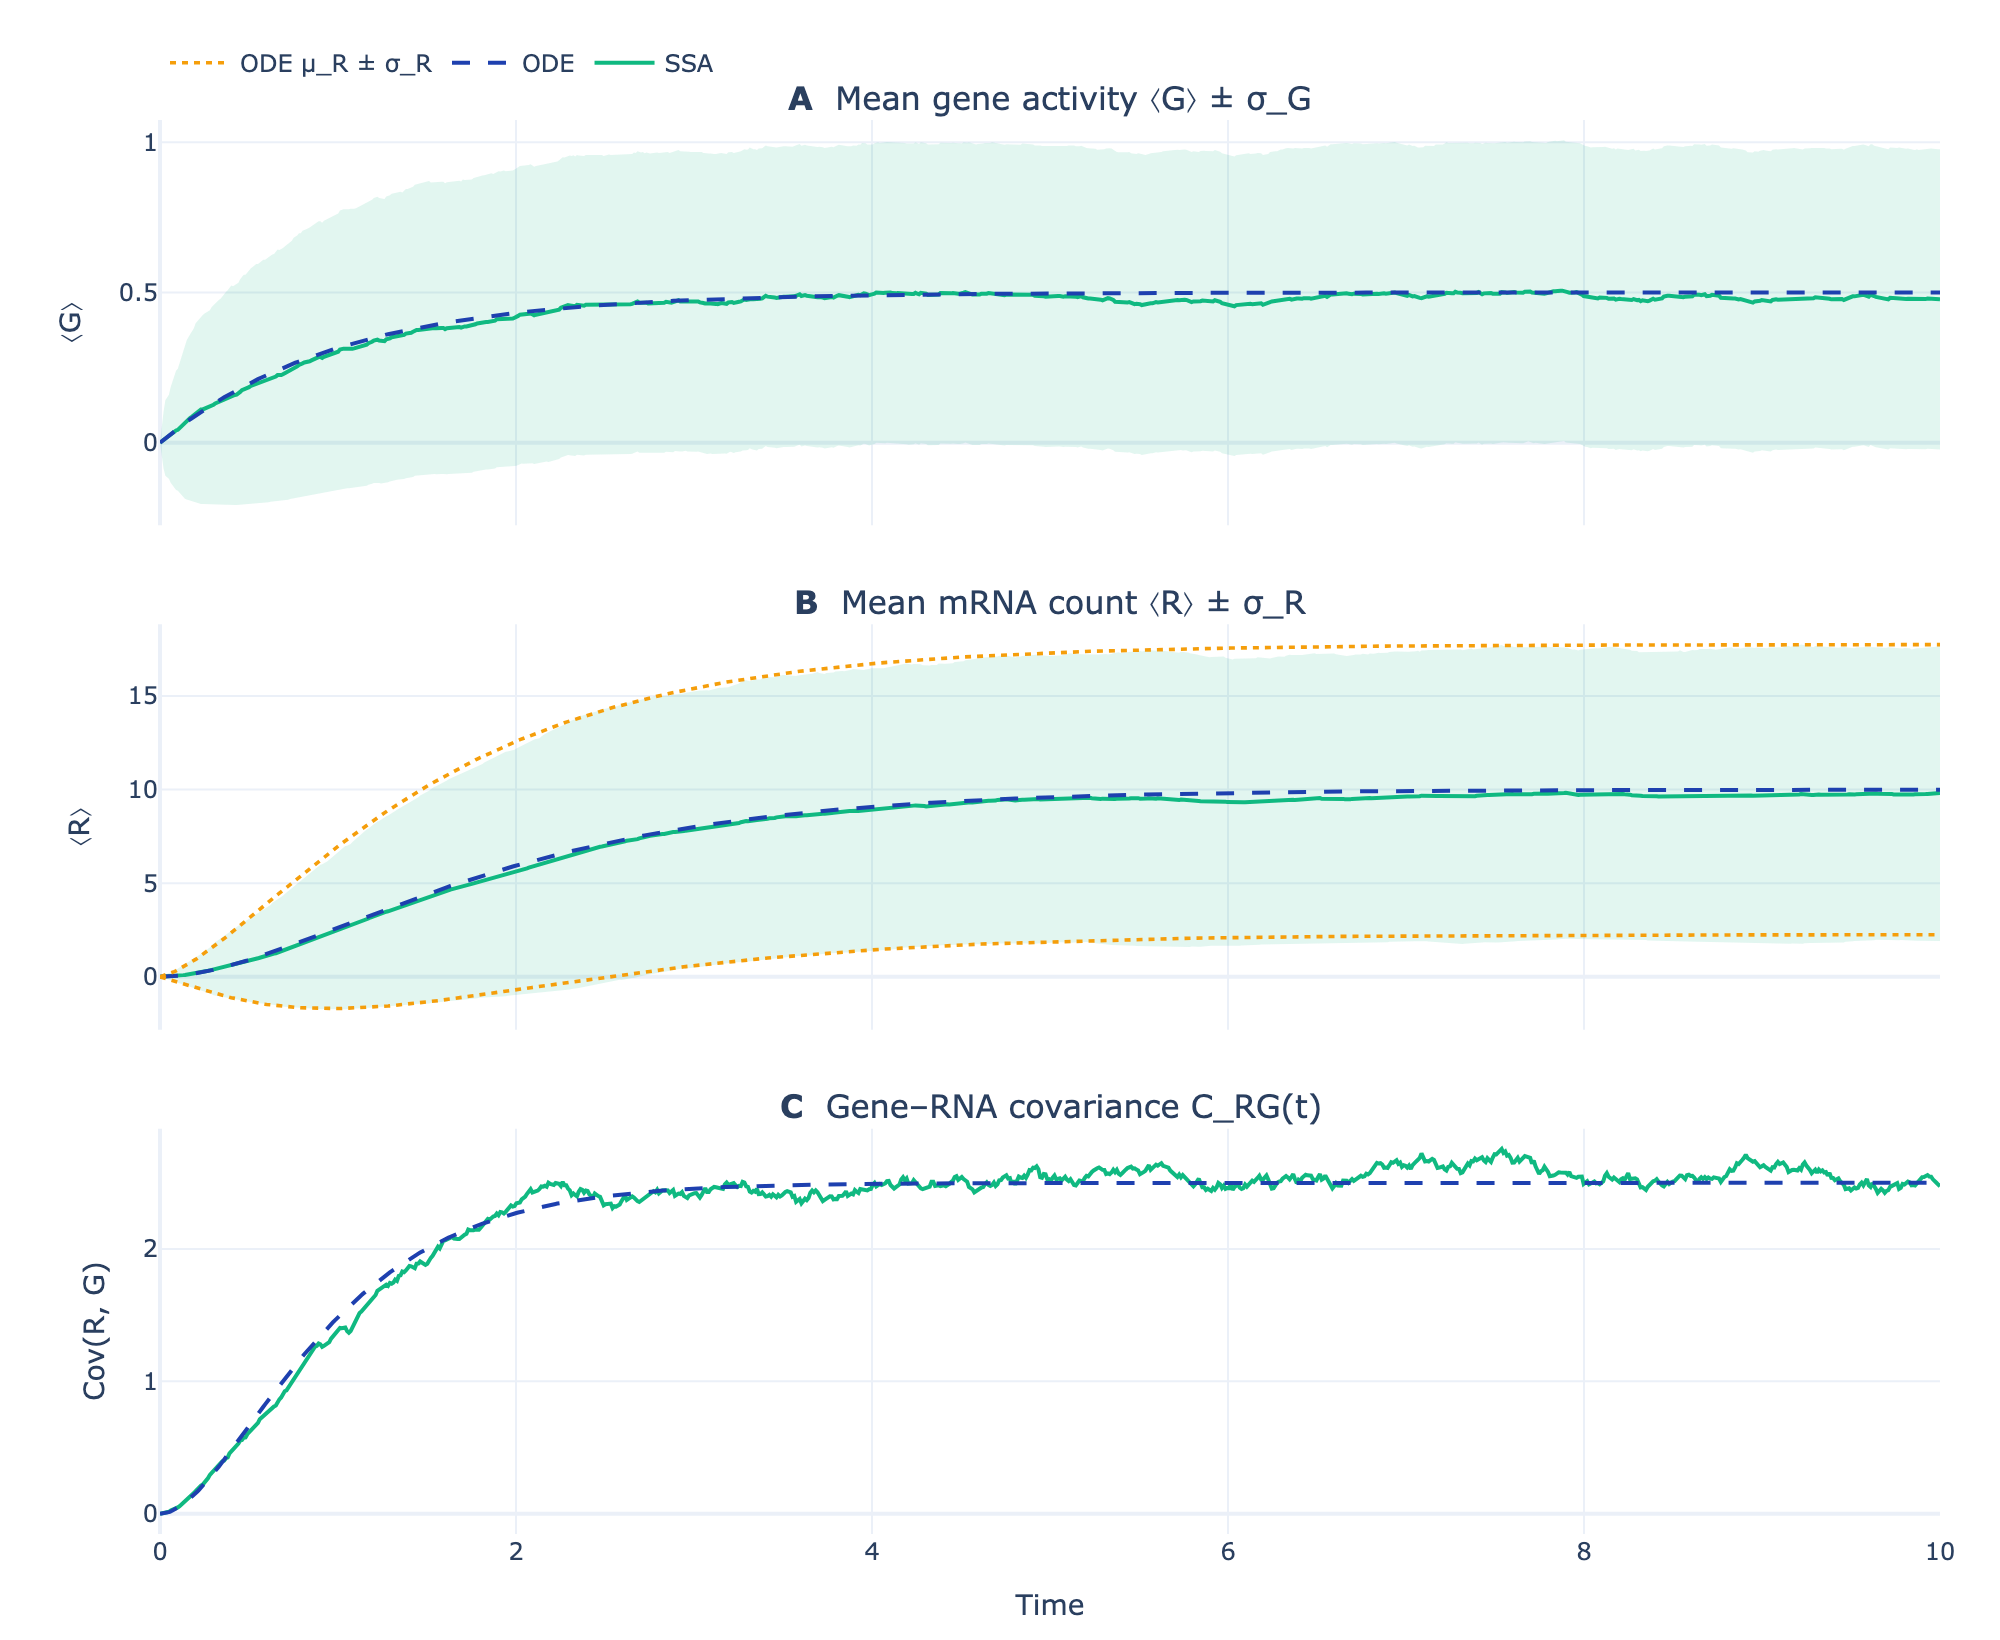
\includegraphics[width=0.9\textwidth]{ssa_vs_ode.png}
  \caption{SSA ensemble averages (green, with the empirical $\pm\sigma$ fluctuation bands shaded)
    and the deterministic ODE solutions (dashed blue) at the reference parameters from
    $(g_0,r_0)=(0,0)$, with $N_{\mathrm{rep}}=1000$. In the mRNA panel the analytical spread from
    the moment ODEs, $\muR\pm\sigma_R$, is drawn as amber dotted lines on top of the SSA band.}
  \label{fig:ssa_vs_ode}
\end{figure}

\begin{figure}[htbp]
  \centering
  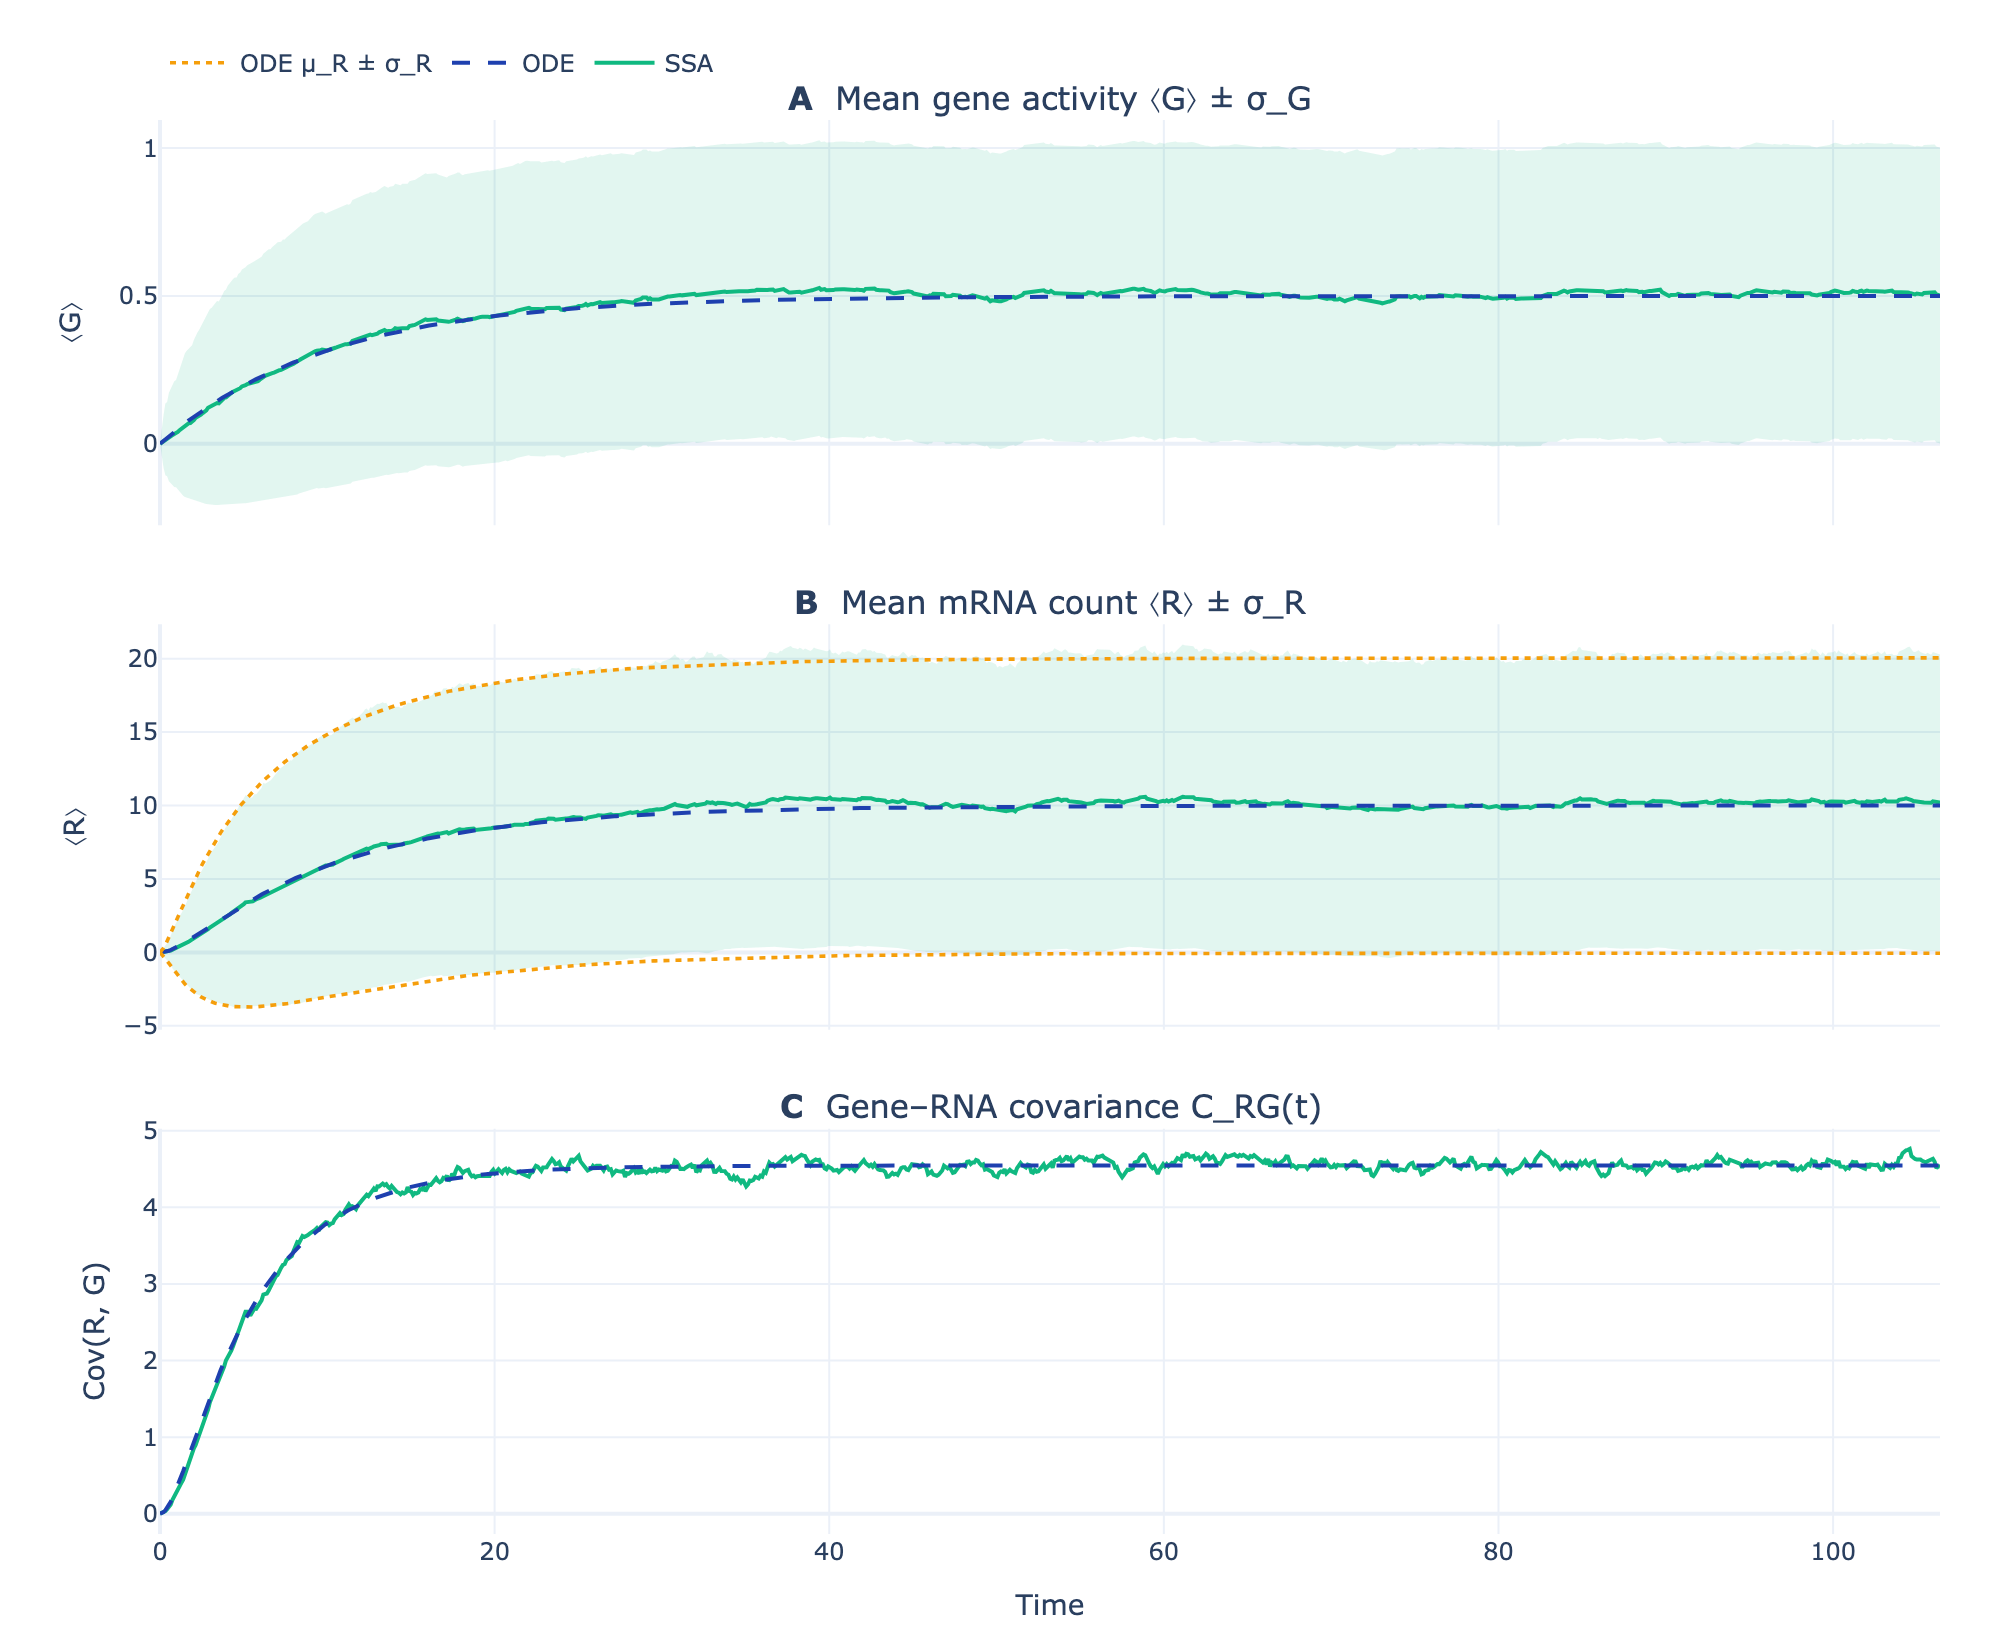
\includegraphics[width=0.85\textwidth]{ssaode_slow.png}
  \caption{SSA versus moment ODEs in the high-noise slow-switching regime. Colours
    are as in Figure~\ref{fig:ssa_vs_ode}: green SSA means with shaded $\pm\sigma$
    bands, dashed blue ODE means, and the amber dotted analytical $\muR\pm\sigma_R$
    overlay in the mRNA panel. Even where fluctuations are largest, the SSA ensemble
    averages track the deterministic ODE curves throughout the transient and into
    steady state, confirming Edge~1 beyond the symmetric reference case.}
  \label{fig:wf-ssaode}
\end{figure}

An overlay, however, is read by eye, and the prediction of
Section~\ref{sec:intersection} is quantitative: the deviation should fall as
$1/\sqrt{N_{\mathrm{rep}}}$. Figure~\ref{fig:edge1_convergence} tests that rate directly. For a
range of ensemble sizes we measure the root-mean-square deviation of $\widehat{\muR}(t)$ from the
ODE curve over the whole time grid (RMS rather than the supremum, an extreme-value statistic that
would not show a clean power law even under exact convergence), and plot it against
$N_{\mathrm{rep}}$ on log--log axes. The
points fall on a straight line of fitted slope $-0.521$ over three decades, against the predicted
$-1/2$. Edge~1 therefore holds not just in the sense that the curves look superimposed at
$N_{\mathrm{rep}}=1000$, but at the rate the Law of Large Numbers requires.

\begin{figure}[htbp]
  \centering
  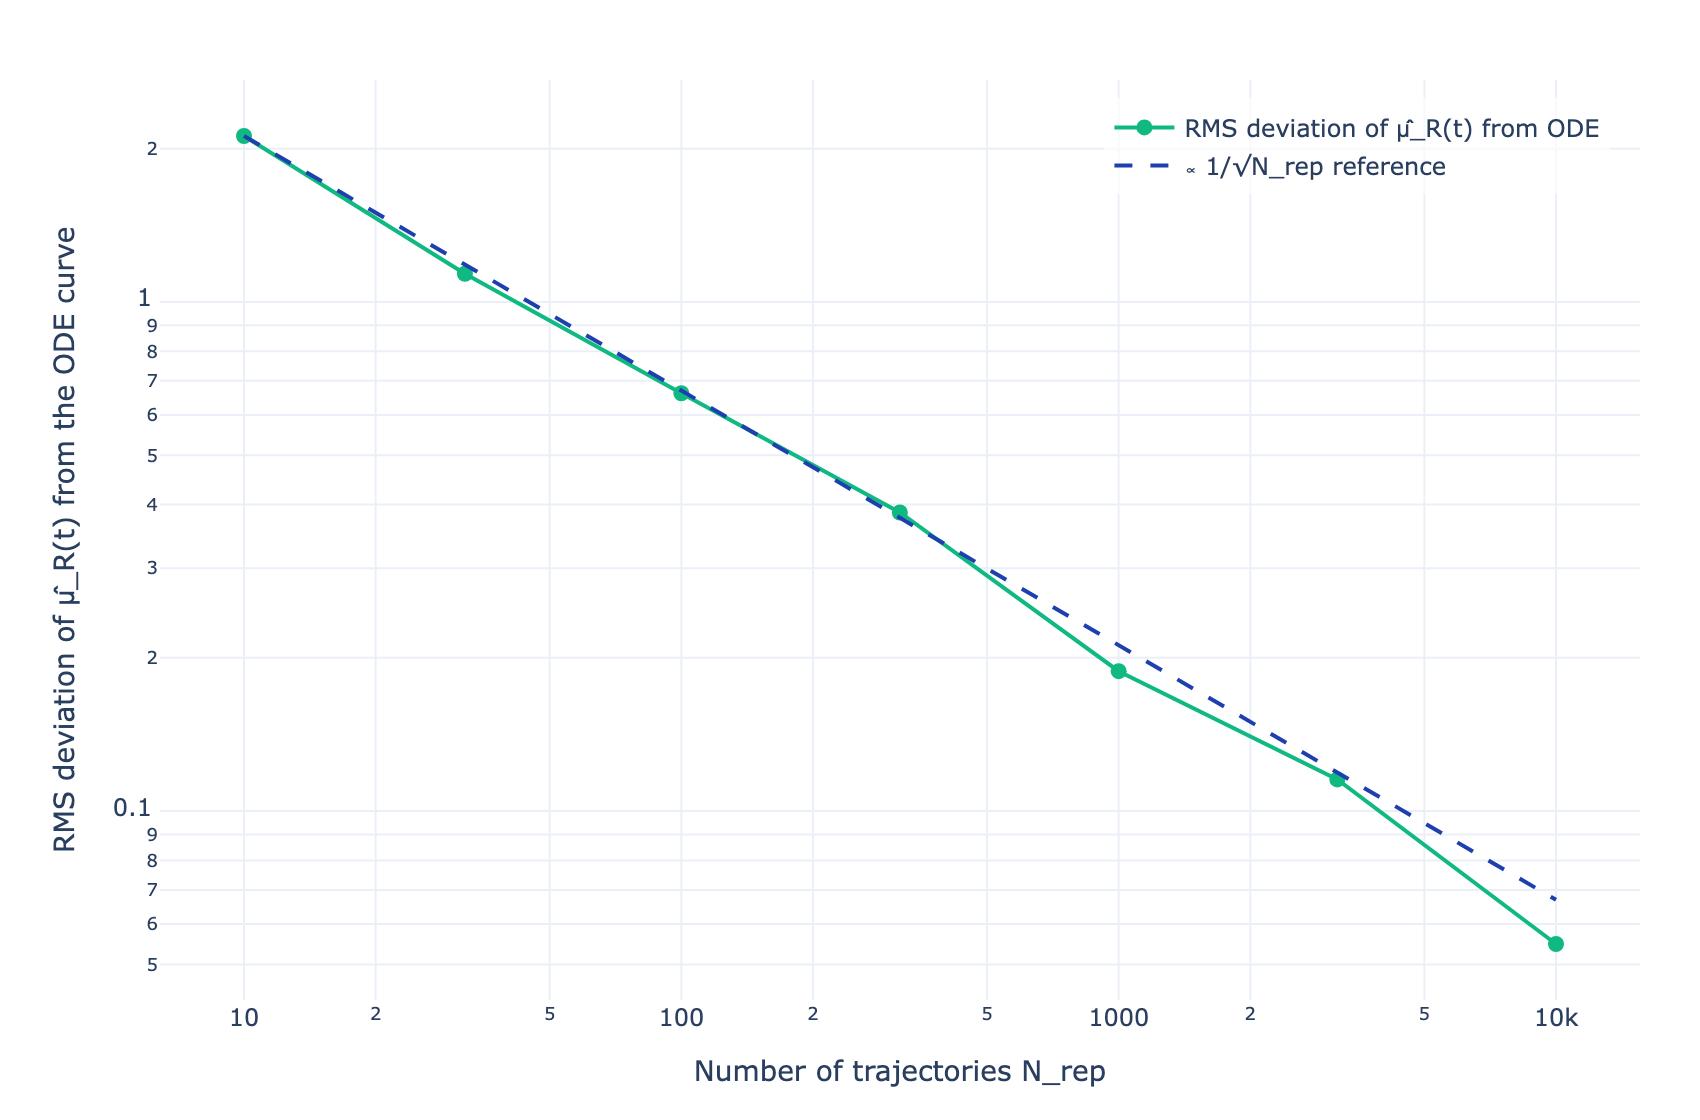
\includegraphics[width=0.8\textwidth]{edge1_convergence.png}
  \caption{Convergence of the SSA ensemble mean to the moment-ODE solution (Edge~1) at the reference
    parameters. The statistic is the RMS deviation of $\widehat{\muR}(t)$ from the ODE curve over the
    full time grid; the dashed line is a $1/\sqrt{N_{\mathrm{rep}}}$ reference anchored at the
    smallest ensemble. The fitted log--log slope is $-0.521$, against the predicted $-1/2$. This is
    the Edge~1 counterpart of Figure~\ref{fig:ss_convergence}, which does the same for Edge~2.}
  \label{fig:edge1_convergence}
\end{figure}

\paragraph{Conclusion.}
The SSA converges to the exact moment dynamics, as predicted by
the Law of Large Numbers, and at the predicted rate, so Edge~1 holds across the regimes tested. The $\pm\sigma$ bands
do \emph{not} collapse onto the mean: they measure genuine cell-to-cell variability,
which persists no matter how many trajectories are averaged and is correctly
predicted by the variance equation~\eqref{eq:dsigR}.

\subsection{Steady-State Validation (Edges 2 \& 3, Notebook 3)}
\label{sec:res-ss}

\paragraph{Aim.}
Verify that the long-time limit of the moment ODEs agrees with the
independent steady-state sampler (Edge~2), that the sampler's error decays at the
Central Limit Theorem rate $1/\sqrt{N_{\mathrm{rep}}}$, that the stationary
\emph{distribution} reached by the SSA is the one the sampler draws from (Edge~3), and that both reduce
correctly to known limits at the boundaries of parameter space (Edge cases).

\paragraph{Result.}
The ODE solutions in Figure~\ref{fig:ssa_vs_ode}
plateau at $\muG^{ss}=0.5$ and $\muR^{ss}=10$, matching the
analytical fixed point~\eqref{eq:ss-means}. The direct sampler reproduces these
values: with $N_{\mathrm{rep}}=2\times10^5$ samples it returns
$\widehat{\muG}^{\,ss}\approx0.5013$ and $\widehat{\muR}^{\,ss}\approx9.976$, agreeing
to within Monte Carlo error: both deviations are well under $1.5$ standard errors, the standard
errors at this sample size being $0.0011$ and $0.017$. Figure~\ref{fig:ss_convergence} makes the convergence
quantitative: on log--log axes, the mean absolute deviation of the sampler's
$\muR^{ss}$ estimate from the exact value follows a line of slope $-\tfrac12$,
matching the $1/\sqrt{N_{\mathrm{rep}}}$ reference over four decades of sample size.

\begin{figure}[htbp]
  \centering
  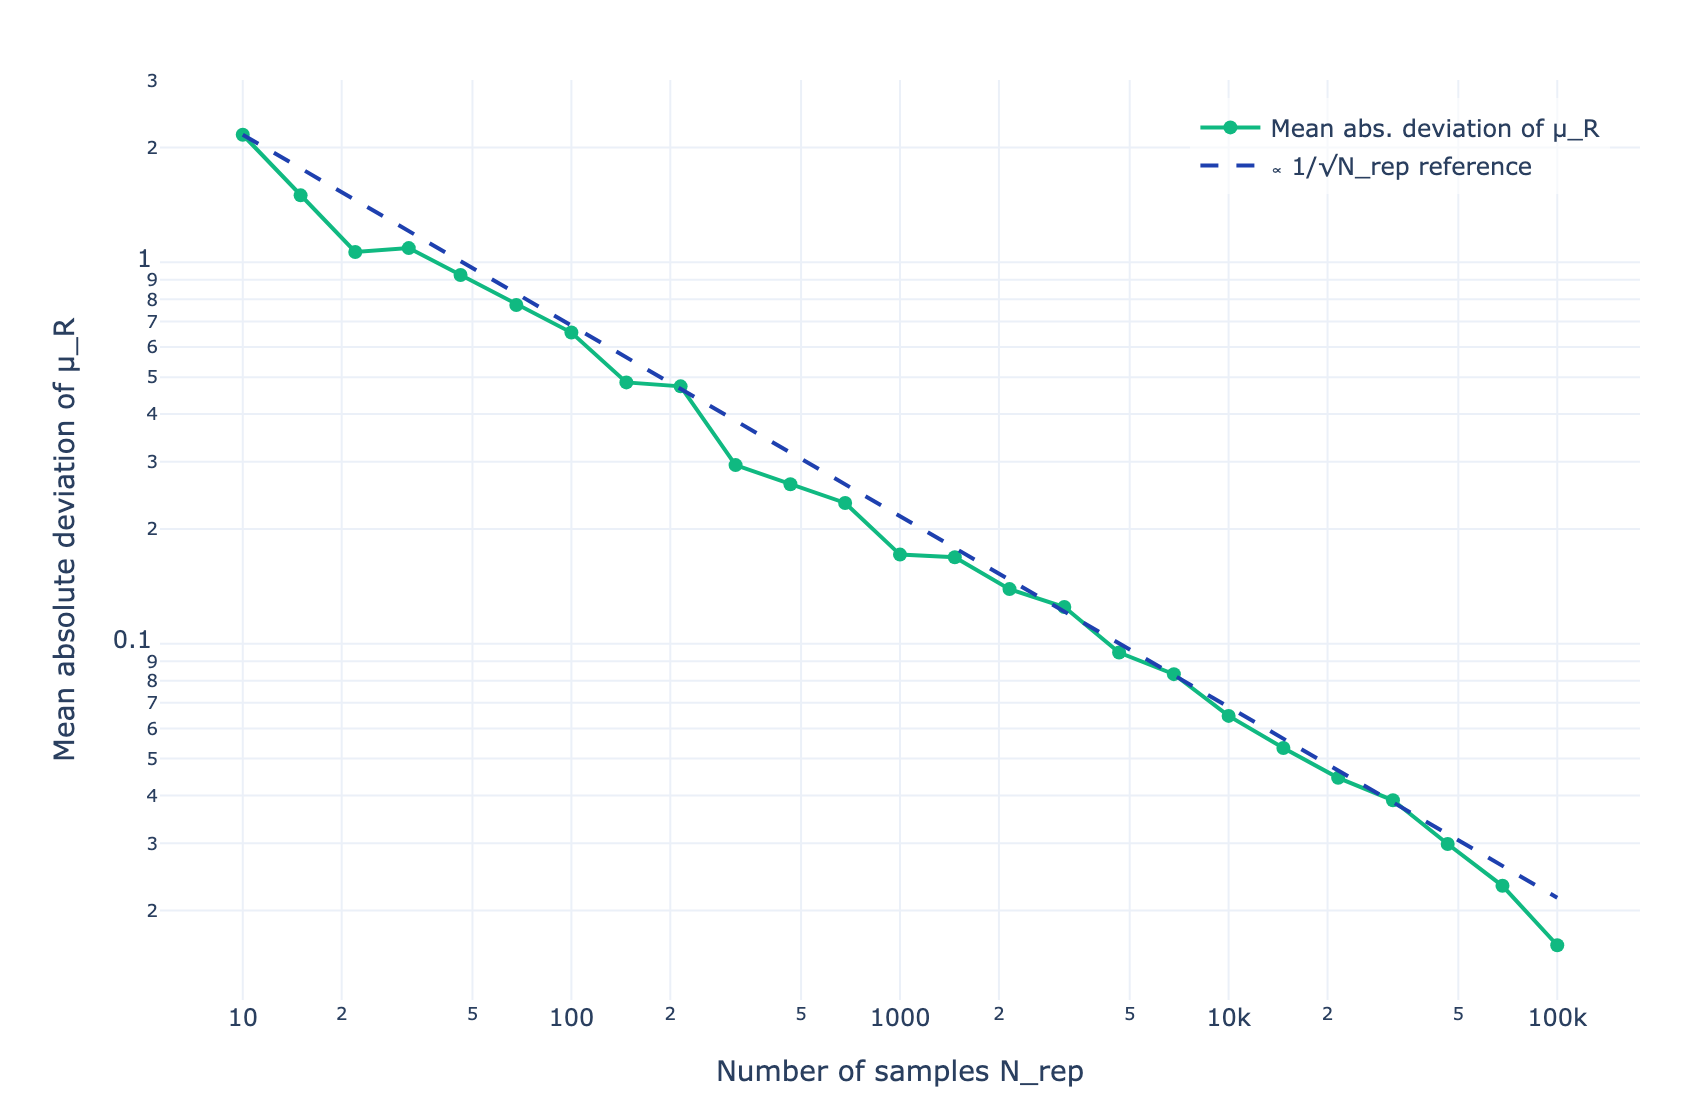
\includegraphics[width=0.8\textwidth]{steady_state_convergence.png}
  \caption{Convergence of the exact steady-state sampler's empirical moments to
    the analytical steady-state values as a function of the number of samples
    $N_{\mathrm{rep}}$. The error (shown as mean absolute deviation) decays as
    $1/\sqrt{N_{\mathrm{rep}}}$, as expected from the Central Limit Theorem.}
  \label{fig:ss_convergence}
\end{figure}

A more demanding check asks the sampler to reproduce \emph{all five} steady-state
moments at once. For $\kon=0.5,\koff=1,\ksyn=20,\kdeg=1$ (so $\muR^{ss}=6.667$), each
moment has a closed form,
\begin{equation}
\label{eq:ss-closed}
  \muG^{ss}=\frac{\kon}{\kon+\koff},\quad
  \muR^{ss}=\frac{\ksyn}{\kdeg}\muG^{ss},\quad
  \CRG^{ss}=\frac{\ksyn\,\muG^{ss}(1-\muG^{ss})}{\kon+\koff+\kdeg},
\end{equation}
together with $\sigma_G^{ss}=\sqrt{\muG^{ss}(1-\muG^{ss})}$ and
$\sigma_R^{ss}=\sqrt{\muR^{ss}+(\ksyn/\kdeg)\,\CRG^{ss}}$. At
$N_{\mathrm{rep}}=2\times10^5$ the sampler matches every moment to within $0.04$
(Table~\ref{tab:moments}), and the absolute error in $\muR$ shows the same
$1/\sqrt{N_{\mathrm{rep}}}$ decay, falling from $3.87$ at $N_{\mathrm{rep}}=10$ to
$0.0145$ at $N_{\mathrm{rep}}=10^5$.

A tolerance such as ``within $0.04$'' is not interpretable on its own, since the moments have
different units and different sampling errors, so the table also reports the Monte Carlo standard
error of each entry. Read in those units, four of the five deviations are well inside one standard
error and $\muR^{ss}$ sits at 2.7---a large but unremarkable fluctuation for a single draw.

\begin{table}[htbp]
  \centering
  \begin{tabular}{lcccc}
  \toprule
  \textbf{Moment} & \textbf{Analytic} & \textbf{Sampler} & \textbf{Abs.\ diff.} & \textbf{Std.\ error} \\
  \midrule
  $\muG^{ss}$    & 0.3333 & 0.3317 & 0.0016 & 0.0010 \\
  $\muR^{ss}$    & 6.6667 & 6.6277 & 0.0389 & 0.0142 \\
  $\sigma_G^{ss}$ & 0.4714 & 0.4708 & 0.0006 & 0.0004 \\
  $\sigma_R^{ss}$ & 6.4979 & 6.4767 & 0.0212 & 0.0105 \\
  $\CRG^{ss}$    & 1.7778 & 1.7666 & 0.0111 & 0.0071 \\
  \bottomrule
  \end{tabular}
  \caption{Steady-state moments from the direct sampler ($N_{\mathrm{rep}}=2\times10^5$)
    against their closed-form values~\eqref{eq:ss-closed}, for
    $\kon=0.5,\koff=1,\ksyn=20,\kdeg=1$. The last column is the Monte Carlo standard error of the
    estimator at this sample size, obtained by bootstrap; for the two means it agrees with the
    closed forms $\sqrt{\muG(1-\muG)/N_{\mathrm{rep}}}$ and
    $\sigma_R/\sqrt{N_{\mathrm{rep}}}$. Because all five moments are computed from a single array of
    Beta draws, their deviations are strongly correlated and are not five independent checks: the
    mean mixing fraction of this draw falls about $0.0016$ low, and since
    $\muR=(\ksyn/\kdeg)\,\overline{p}$ multiplies that shortfall by $20$, it accounts for $0.032$ of
    the $0.039$ observed in $\muR^{ss}$. One fluctuation is being reported five times.}
  \label{tab:moments}
\end{table}

Finally, we test the two limits where the model reduces to a known result, including
the $\koff=0$ prediction made in Section~\ref{sec:ss}. When the gene
never switches off, it is permanently active and the telegraph model
reduces to a birth--death process---a Markov chain whose only moves are $+1$ and
$-1$---whose stationary law is a Poisson distribution~\cite{vankampen,gardiner}; the moment ODEs accordingly
relax to $\muG^{ss}=1$, $\muR^{ss}=\ksyn/\kdeg$. Figure~\ref{fig:wf-poisson} overlays
the sampled counts on the analytic Poisson PMF; they coincide, with $\muR\approx9.99$
and a Fano factor (the variance-to-mean ratio) $\approx0.99$, against the expected
mean $\ksyn/\kdeg=10$ and Fano factor $1$. In the opposite limit, with no degradation
($\kdeg=0$), mRNA accumulates without bound and no steady state exists; the sampler
detects this and raises a \texttt{ValueError} instead of returning an invalid result.

\paragraph{Edge 3 as a distributional test.}
Two different laws can share a mean, a variance and a covariance, and this paper claims that the
three \emph{descriptions} agree, not merely their first two moments. Since both endpoints of Edge~3
produce samples, we can compare the full stationary distributions directly.

Figure~\ref{fig:edge3} does this in two regimes. In each, $20\,000$ independent SSA trajectories are
run far past stationarity and the mRNA count is read off at a single late time---one draw per
replicate, never pooled over a time window, whose successive samples are autocorrelated and would
understate the spread. That histogram is compared with $2\times10^5$ draws from the steady-state
sampler. The discrepancy is measured in total variation,
$\mathrm{TV}=\tfrac12\sum_r|\hat P^{\mathrm{SSA}}(r)-\hat P^{\mathrm{smp}}(r)|$, which needs no
binning, is bounded in $[0,1]$, and reads directly as the largest probability the two laws can
assign differently to any event---where a $\chi^2$ test would force an arbitrary merge of the
near-empty bins in the trough of the slow-switching law.

The null band is obtained by \emph{direct resimulation}: under the null hypothesis the stationary
law the SSA samples is exactly the law the sampler draws from, so we simply draw $200$ fresh pairs
at the same two sample sizes and recompute TV. This is the null the test actually claims, and it
needs no resampling approximation. The obvious alternative---bootstrapping each side from its own
empirical measure---does not estimate it: that adds sampling noise twice over and centres the band
above the TV expected under the null, so a passing test is flattered by a band that is too wide.
(A pooled two-sample permutation null does reproduce the correct band, its median falling within
$2\%$ of the resimulated one, but direct simulation is cheaper here and free of the subtlety.)

The slow-switching panel is the demanding one, and it is where the moments are least informative.
There the exact stationary law is strongly bimodal: mass piles up at $R=0$ (a gene that has been OFF
for a long time) and near $R=\ksyn/\kdeg=20$ (one that has been ON), while the mean $\muR=10$ falls
in the trough between them, roughly fifty times less likely than $R=0$. A method could match
$\muR$ and $\sigma_R$ exactly and still get this shape wrong, so the $\pm\sigma$ bands drawn
elsewhere in this paper---correct as summaries---invite a Gaussian reading that the underlying law
does not support. Measured this way the two distributions agree. In the symmetric regime the observed
$\mathrm{TV}=0.0093$ against a null median of $0.0155$ and 95th percentile of $0.0191$; in the slow
regime, $\mathrm{TV}=0.0117$ against a median of $0.0130$ and 95th percentile of $0.0166$. The
one-sided $p$-values---the null fraction at least as large as the observed TV---are $1.00$ and
$0.74$, so neither regime shows a discrepancy beyond chance.

The symmetric value sits below every one of the $200$ null draws, which is a low result rather than
an impossible one, and it is worth saying why we read it that way. The SSA sample there is simply a
central draw: its variance, $59.8$, matches the analytic
$\sigRsq=\muR+(\ksyn/\kdeg)\,\CRG=60$ to $0.4\%$, and splitting it in half reproduces the dispersion
of two independent sampler draws of the same size. The agreement is therefore fortunate in its
magnitude but not anomalous in kind. The test could have failed---the band is narrow enough that a
TV of $0.03$ would have been unambiguous---and it puts the weight on the SSA, the hand-written
nested loop of this project and its most error-prone component, where the sampler is three
vectorised NumPy calls whose moments were verified symbolically in Section~\ref{sec:ss}.

\begin{figure}[htbp]
  \centering
  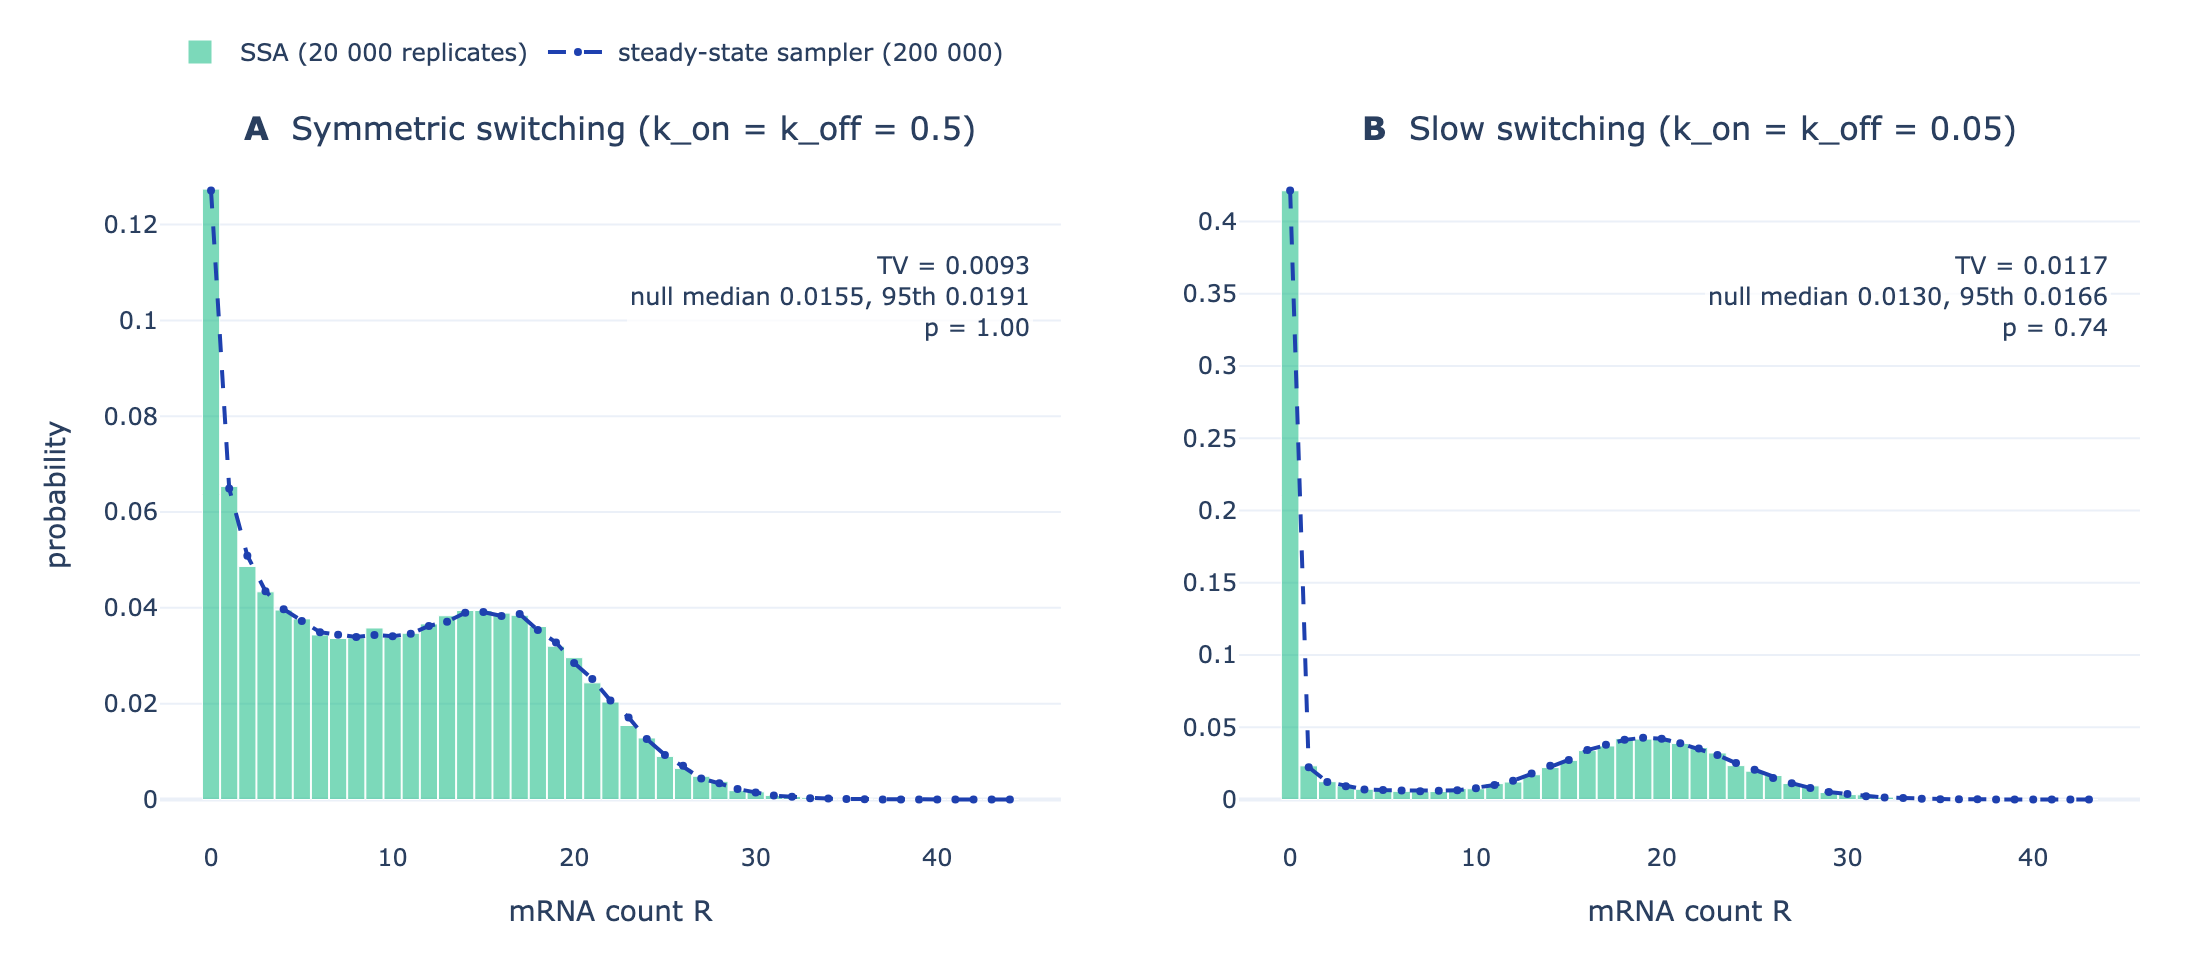
\includegraphics[width=\textwidth]{edge3_distribution.png}
  \caption{Edge~3 as a distributional test: the stationary mRNA distribution from $20\,000$
    independent SSA trajectories (green bars, read at one late time per replicate) against
    $2\times10^5$ draws from the steady-state sampler (dashed blue). Left: the symmetric reference
    regime. Right: slow switching ($\kon=\koff=0.05$), where the exact law is bimodal, with modes at
    $R=0$ and near $R=\ksyn/\kdeg=20$ and a trough at the mean $\muR=10$. Each panel gives the
    observed total-variation distance with the median and 95th percentile of the resimulated null
    band and the one-sided $p$-value.}
  \label{fig:edge3}
\end{figure}

\begin{figure}[htbp]
  \centering
  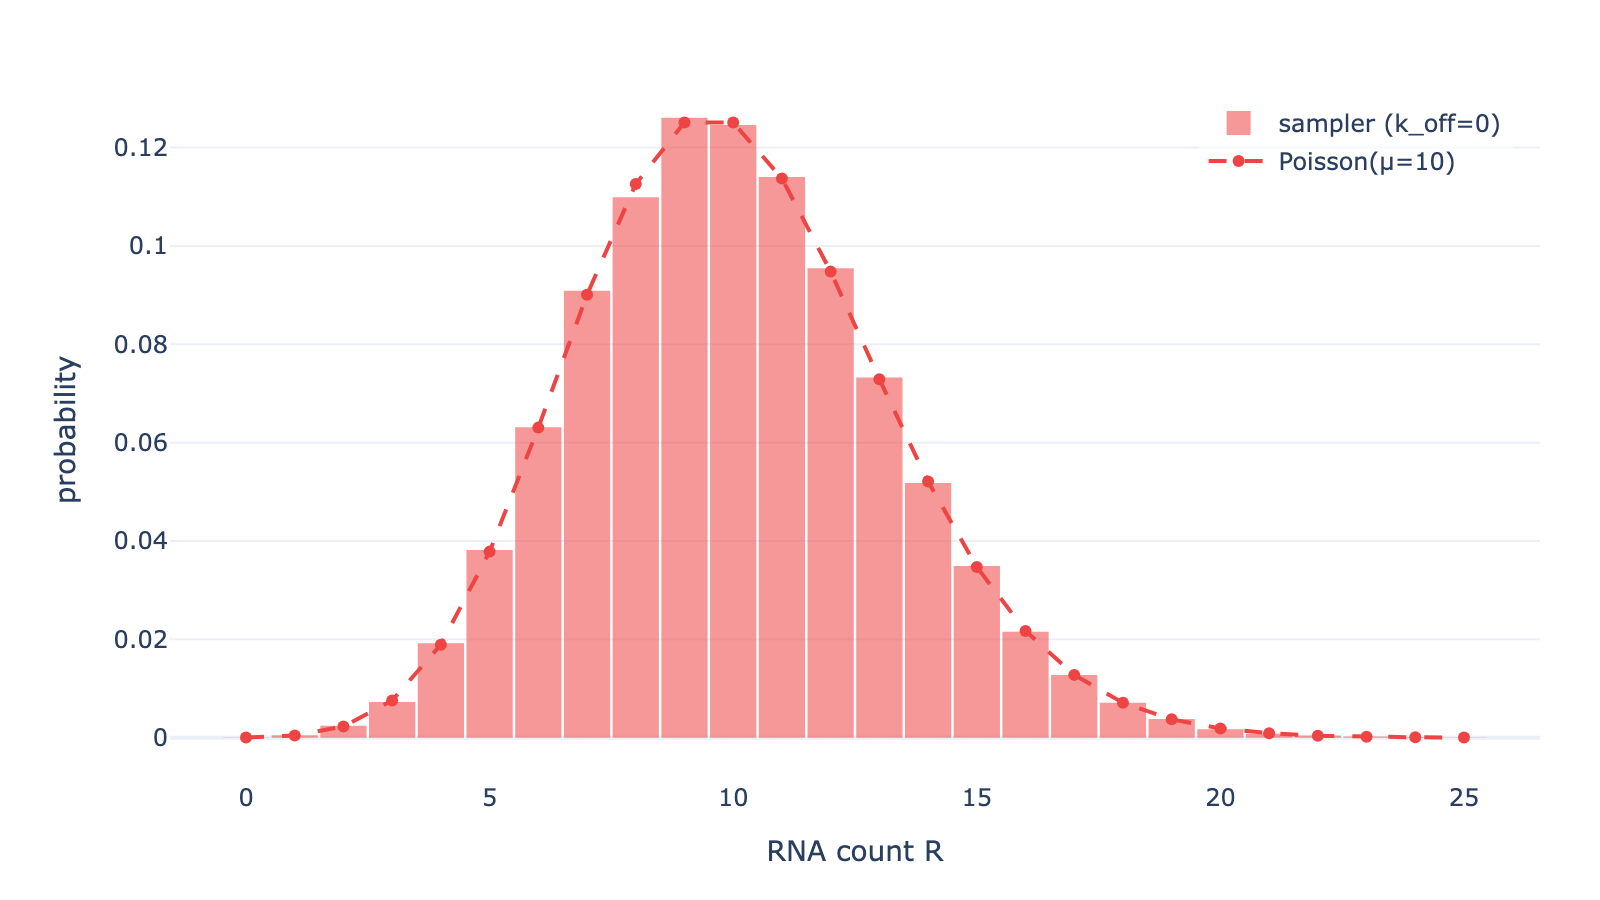
\includegraphics[width=0.7\textwidth]{validation_poisson.png}
  \caption{Edge case $\koff=0$ (permanently active gene). The sampled
    steady-state mRNA distribution matches the analytic Poisson PMF with mean
    $\ksyn/\kdeg=10$ (Fano factor $\approx1$), the exact limit the telegraph model
    must reduce to when the gene never switches off.}
  \label{fig:wf-poisson}
\end{figure}

\paragraph{Conclusion.}
The sampler is an unbiased, $\sqrt{N}$-consistent estimator of the
steady-state moments, so Edge~2 holds. Edge~3 holds independently rather than by inheritance from
the other two: the SSA moments (Figure~\ref{fig:ssa_vs_ode}) plateau at the same values, and
Figure~\ref{fig:edge3} shows that the agreement extends to the whole stationary distribution, in a
comparison that had room to fail. With that, the three edges close the triangle, establishing mutual
consistency of the
stochastic, deterministic, and stationary descriptions---at the level of moments on two edges, and
of the full law on the third. The correct behaviour at the
$\koff=0$ and $\kdeg=0$ boundaries shows the agreement is not an artifact of the
particular parameter set.

\FloatBarrier
\section{Conclusion}
\label{sec:conclusion}

We have studied the telegraph model of stochastic gene expression from three
mathematically distinct viewpoints---exact stochastic simulation, closed moment
ODEs, and direct steady-state sampling---and shown that they agree. 
Each way was confirmed numerically to within the expected
$1/\sqrt{N_{\mathrm{rep}}}$ statistical error, and the methods were further
validated on solvable edge cases.

Beyond verifying three correct implementations, this illustrates a general principle: when the same
system can be described at several levels of abstraction, those descriptions become mutual tests.
The limits of what was checked are worth stating. Only the marginal law of $R$ was compared as a
distribution; the joint law of $(G,R)$ was tested at the level of moments alone, and the transient
was never compared as a distribution, only through its first two moments.

\section{Future Work}
\label{sec:future}

The telegraph model is a starting point, and two extensions would make it more realistic.

\paragraph{Adding the protein level.}
mRNA is only an intermediate: it is translated into protein, which is usually what the cell actually
uses. A natural next step is a three-stage model, gene $\to$ mRNA $\to$ protein, with two extra
reactions: translation of protein from mRNA at rate $k_{\mathrm{trans}}$, and protein degradation at
rate $k_{\mathrm{deg},p}$. The same tools carry over directly---the SSA simply gains two reactions,
and the moment ODEs gain equations for the mean and variance of the protein count and its covariance
with mRNA---so we could follow how noise is passed from the gene down to the protein, the level at
which most measurements are made.

\paragraph{Networks of interacting genes.}
Real genes do not act alone: the protein made by one gene can switch another gene ON or OFF, forming
a \emph{gene regulatory network}. A compact way to describe such a network is to treat each gene's
ON/OFF state as a spin in an \emph{Ising model}, where ON and OFF play the role of the two spin
states and the regulatory links act as couplings between spins. The obstacle is dimensionality: with
$n$ genes the joint distribution has $2^n$ gene configurations (times all the mRNA and protein
counts), far too many to store or integrate directly. Here \emph{machine-learning} methods---for
example neural-network density estimators or variational approximations---give a practical way to
approximate these high-dimensional probability distributions, learning a compact model of the
stationary state instead of enumerating it. Combining the exact small-system checks of this paper
with such approximate large-system methods is a promising direction.

\begin{thebibliography}{99}

\bibitem{gillespie1976}
D.~T.~Gillespie,
\textit{A general method for numerically simulating the stochastic time evolution
of coupled chemical reactions},
Journal of Computational Physics \textbf{22} (1976), no.~4, 403--434.

\bibitem{gillespie1977}
D.~T.~Gillespie,
\textit{Exact stochastic simulation of coupled chemical reactions},
Journal of Physical Chemistry \textbf{81} (1977), no.~25, 2340--2361.

\bibitem{gillespie2007}
D.~T.~Gillespie,
\textit{Stochastic simulation of chemical kinetics},
Annual Review of Physical Chemistry \textbf{58} (2007), no.~1, 35--55.
Open-access copy: \href{https://pmc.ncbi.nlm.nih.gov/articles/PMC7610481/}{PMC7610481}.
\textit{(Review of exact and approximate stochastic simulation algorithms for
chemical reaction systems; background for the SSA used here.)}

\bibitem{peccoud1995}
J.~Peccoud and B.~Ycart,
\textit{Markovian modeling of gene-product synthesis},
Theoretical Population Biology \textbf{48} (1995), no.~2, 222--234.
\textit{(Derives the stationary Beta--Poisson distribution of the two-state
telegraph model; basis for the steady-state sampler.)}

\bibitem{raj2006}
A.~Raj, C.~S.~Peskin, D.~Tranchina, D.~Y.~Vargas, and S.~Tyagi,
\textit{Stochastic mRNA synthesis in mammalian cells},
PLoS Biology \textbf{4} (2006), no.~10, e309.
\textit{(Single-molecule mRNA counts showing bursty, over-dispersed expression
consistent with the telegraph model.)}

\bibitem{elowitz2002}
M.~B.~Elowitz, A.~J.~Levine, E.~D.~Siggia, and P.~S.~Swain,
\textit{Stochastic gene expression in a single cell},
Science \textbf{297} (2002), no.~5584, 1183--1186.
\textit{(Separates intrinsic from extrinsic noise in single cells; source for the
noise decomposition stated in the Introduction.)}

\bibitem{ozbudak2002}
E.~M.~Ozbudak, M.~Thattai, I.~Kurtser, A.~D.~Grossman, and A.~van Oudenaarden,
\textit{Regulation of noise in the expression of a single gene},
Nature Genetics \textbf{31} (2002), no.~1, 69--73.
\textit{(Measures how transcription and translation rates set expression noise in a
single gene.)}

\bibitem{ko1991}
M.~S.~H.~Ko,
\textit{A stochastic model for gene induction},
Journal of Theoretical Biology \textbf{153} (1991), no.~2, 181--194.
\textit{(Introduces the two-state ON/OFF gene model underlying the telegraph model
used here.)}

\bibitem{fano1947}
U.~Fano,
\textit{Ionization yield of radiations. II. The fluctuations of the number of ions},
Physical Review \textbf{72} (1947), no.~1, 26--29.
\textit{(Origin of the variance-to-mean ratio now called the Fano factor.)}

\bibitem{golding2005}
I.~Golding, J.~Paulsson, S.~M.~Zawilski, and E.~C.~Cox,
\textit{Real-time kinetics of gene activity in individual bacteria},
Cell \textbf{123} (2005), no.~6, 1025--1036.
\textit{(Direct observation of transcriptional bursts in single bacteria; empirical
support for the burst picture.)}

\bibitem{iyerbiswas2009}
S.~Iyer-Biswas, F.~Hayot, and C.~Jayaprakash,
\textit{Stochasticity of gene products from transcriptional pulsing},
Physical Review E \textbf{79} (2009), no.~3, 031911.
\textit{(Exact time-dependent solution of the master equation for the two-state
pulsing gene; reference for the fast- and slow-switching limits.)}

\bibitem{schnoerr2015}
D.~Schnoerr, G.~Sanguinetti, and R.~Grima,
\textit{Comparison of different moment-closure approximations for stochastic
chemical kinetics},
Journal of Chemical Physics \textbf{143} (2015), no.~18, 185101.
\textit{(Survey of approximate closure schemes needed when the moment hierarchy does
not close --- the situation avoided exactly in this paper.)}

\bibitem{vankampen}
N.~G.~van Kampen,
\textit{Stochastic Processes in Physics and Chemistry},
3rd ed., North-Holland, Amsterdam, 2007.

\bibitem{gardiner}
C.~W.~Gardiner,
\textit{Handbook of Stochastic Methods for Physics, Chemistry and the Natural
Sciences},
3rd ed., Springer, Berlin, 2004.

\bibitem{wilkinson}
D.~J.~Wilkinson,
\textit{Stochastic Modelling for Systems Biology},
2nd ed., Chapman \& Hall/CRC Mathematical and Computational Biology Series, Boca Raton, 2011.
\textit{(Textbook on the chemical master equation and stochastic simulation of
biochemical networks; reference for the CME and the SSA.)}

\bibitem{ingalls}
B.~P.~Ingalls,
\textit{Mathematical Modelling in Systems Biology: An Introduction},
University of Waterloo, 2012.
\textit{(Introductory text on deterministic and stochastic models of biochemical
and gene-regulatory systems; reference for the moment ODEs.)}

\bibitem{harris2020}
C.~R.~Harris et al.,
\textit{Array programming with NumPy},
Nature \textbf{585} (2020), no.~7825, 357--362.
\textit{(NumPy; array computation and the random number generation used throughout.)}

\bibitem{virtanen2020}
P.~Virtanen et al.,
\textit{SciPy 1.0: fundamental algorithms for scientific computing in Python},
Nature Methods \textbf{17} (2020), no.~3, 261--272.
\textit{(SciPy; provides the \texttt{solve\_ivp} integrator used for the moment ODEs.)}

\bibitem{dormand1980}
J.~R.~Dormand and P.~J.~Prince,
\textit{A family of embedded Runge--Kutta formulae},
Journal of Computational and Applied Mathematics \textbf{6} (1980), no.~1, 19--26.
\textit{(The embedded Runge--Kutta pair implemented as the \texttt{RK45} method.)}

\bibitem{matsumoto1998}
M.~Matsumoto and T.~Nishimura,
\textit{Mersenne Twister: a 623-dimensionally equidistributed uniform pseudo-random
number generator},
ACM Transactions on Modeling and Computer Simulation \textbf{8} (1998), no.~1, 3--30.
\textit{(The MT19937 generator supplying every pseudo-random draw in this work.)}

\end{thebibliography}

\end{document}
